% Options for packages loaded elsewhere
\PassOptionsToPackage{unicode}{hyperref}
\PassOptionsToPackage{hyphens}{url}
%
\documentclass[
  letterpaper,
]{scrbook}

\usepackage{amsmath,amssymb}
\usepackage{iftex}
\ifPDFTeX
  \usepackage[T1]{fontenc}
  \usepackage[utf8]{inputenc}
  \usepackage{textcomp} % provide euro and other symbols
\else % if luatex or xetex
  \usepackage{unicode-math}
  \defaultfontfeatures{Scale=MatchLowercase}
  \defaultfontfeatures[\rmfamily]{Ligatures=TeX,Scale=1}
\fi
\usepackage{lmodern}
\ifPDFTeX\else  
    % xetex/luatex font selection
\fi
% Use upquote if available, for straight quotes in verbatim environments
\IfFileExists{upquote.sty}{\usepackage{upquote}}{}
\IfFileExists{microtype.sty}{% use microtype if available
  \usepackage[]{microtype}
  \UseMicrotypeSet[protrusion]{basicmath} % disable protrusion for tt fonts
}{}
\makeatletter
\@ifundefined{KOMAClassName}{% if non-KOMA class
  \IfFileExists{parskip.sty}{%
    \usepackage{parskip}
  }{% else
    \setlength{\parindent}{0pt}
    \setlength{\parskip}{6pt plus 2pt minus 1pt}}
}{% if KOMA class
  \KOMAoptions{parskip=half}}
\makeatother
\usepackage{xcolor}
\ifLuaTeX
  \usepackage{luacolor}
  \usepackage[soul]{lua-ul}
\else
  \usepackage{soul}
  
\fi
\setlength{\emergencystretch}{3em} % prevent overfull lines
\setcounter{secnumdepth}{-\maxdimen} % remove section numbering
% Make \paragraph and \subparagraph free-standing
\makeatletter
\ifx\paragraph\undefined\else
  \let\oldparagraph\paragraph
  \renewcommand{\paragraph}{
    \@ifstar
      \xxxParagraphStar
      \xxxParagraphNoStar
  }
  \newcommand{\xxxParagraphStar}[1]{\oldparagraph*{#1}\mbox{}}
  \newcommand{\xxxParagraphNoStar}[1]{\oldparagraph{#1}\mbox{}}
\fi
\ifx\subparagraph\undefined\else
  \let\oldsubparagraph\subparagraph
  \renewcommand{\subparagraph}{
    \@ifstar
      \xxxSubParagraphStar
      \xxxSubParagraphNoStar
  }
  \newcommand{\xxxSubParagraphStar}[1]{\oldsubparagraph*{#1}\mbox{}}
  \newcommand{\xxxSubParagraphNoStar}[1]{\oldsubparagraph{#1}\mbox{}}
\fi
\makeatother

\usepackage{color}
\usepackage{fancyvrb}
\newcommand{\VerbBar}{|}
\newcommand{\VERB}{\Verb[commandchars=\\\{\}]}
\DefineVerbatimEnvironment{Highlighting}{Verbatim}{commandchars=\\\{\}}
% Add ',fontsize=\small' for more characters per line
\usepackage{framed}
\definecolor{shadecolor}{RGB}{241,243,245}
\newenvironment{Shaded}{\begin{snugshade}}{\end{snugshade}}
\newcommand{\AlertTok}[1]{\textcolor[rgb]{0.68,0.00,0.00}{#1}}
\newcommand{\AnnotationTok}[1]{\textcolor[rgb]{0.37,0.37,0.37}{#1}}
\newcommand{\AttributeTok}[1]{\textcolor[rgb]{0.40,0.45,0.13}{#1}}
\newcommand{\BaseNTok}[1]{\textcolor[rgb]{0.68,0.00,0.00}{#1}}
\newcommand{\BuiltInTok}[1]{\textcolor[rgb]{0.00,0.23,0.31}{#1}}
\newcommand{\CharTok}[1]{\textcolor[rgb]{0.13,0.47,0.30}{#1}}
\newcommand{\CommentTok}[1]{\textcolor[rgb]{0.37,0.37,0.37}{#1}}
\newcommand{\CommentVarTok}[1]{\textcolor[rgb]{0.37,0.37,0.37}{\textit{#1}}}
\newcommand{\ConstantTok}[1]{\textcolor[rgb]{0.56,0.35,0.01}{#1}}
\newcommand{\ControlFlowTok}[1]{\textcolor[rgb]{0.00,0.23,0.31}{\textbf{#1}}}
\newcommand{\DataTypeTok}[1]{\textcolor[rgb]{0.68,0.00,0.00}{#1}}
\newcommand{\DecValTok}[1]{\textcolor[rgb]{0.68,0.00,0.00}{#1}}
\newcommand{\DocumentationTok}[1]{\textcolor[rgb]{0.37,0.37,0.37}{\textit{#1}}}
\newcommand{\ErrorTok}[1]{\textcolor[rgb]{0.68,0.00,0.00}{#1}}
\newcommand{\ExtensionTok}[1]{\textcolor[rgb]{0.00,0.23,0.31}{#1}}
\newcommand{\FloatTok}[1]{\textcolor[rgb]{0.68,0.00,0.00}{#1}}
\newcommand{\FunctionTok}[1]{\textcolor[rgb]{0.28,0.35,0.67}{#1}}
\newcommand{\ImportTok}[1]{\textcolor[rgb]{0.00,0.46,0.62}{#1}}
\newcommand{\InformationTok}[1]{\textcolor[rgb]{0.37,0.37,0.37}{#1}}
\newcommand{\KeywordTok}[1]{\textcolor[rgb]{0.00,0.23,0.31}{\textbf{#1}}}
\newcommand{\NormalTok}[1]{\textcolor[rgb]{0.00,0.23,0.31}{#1}}
\newcommand{\OperatorTok}[1]{\textcolor[rgb]{0.37,0.37,0.37}{#1}}
\newcommand{\OtherTok}[1]{\textcolor[rgb]{0.00,0.23,0.31}{#1}}
\newcommand{\PreprocessorTok}[1]{\textcolor[rgb]{0.68,0.00,0.00}{#1}}
\newcommand{\RegionMarkerTok}[1]{\textcolor[rgb]{0.00,0.23,0.31}{#1}}
\newcommand{\SpecialCharTok}[1]{\textcolor[rgb]{0.37,0.37,0.37}{#1}}
\newcommand{\SpecialStringTok}[1]{\textcolor[rgb]{0.13,0.47,0.30}{#1}}
\newcommand{\StringTok}[1]{\textcolor[rgb]{0.13,0.47,0.30}{#1}}
\newcommand{\VariableTok}[1]{\textcolor[rgb]{0.07,0.07,0.07}{#1}}
\newcommand{\VerbatimStringTok}[1]{\textcolor[rgb]{0.13,0.47,0.30}{#1}}
\newcommand{\WarningTok}[1]{\textcolor[rgb]{0.37,0.37,0.37}{\textit{#1}}}

\providecommand{\tightlist}{%
  \setlength{\itemsep}{0pt}\setlength{\parskip}{0pt}}\usepackage{longtable,booktabs,array}
\usepackage{calc} % for calculating minipage widths
% Correct order of tables after \paragraph or \subparagraph
\usepackage{etoolbox}
\makeatletter
\patchcmd\longtable{\par}{\if@noskipsec\mbox{}\fi\par}{}{}
\makeatother
% Allow footnotes in longtable head/foot
\IfFileExists{footnotehyper.sty}{\usepackage{footnotehyper}}{\usepackage{footnote}}
\makesavenoteenv{longtable}
\usepackage{graphicx}
\makeatletter
\newsavebox\pandoc@box
\newcommand*\pandocbounded[1]{% scales image to fit in text height/width
  \sbox\pandoc@box{#1}%
  \Gscale@div\@tempa{\textheight}{\dimexpr\ht\pandoc@box+\dp\pandoc@box\relax}%
  \Gscale@div\@tempb{\linewidth}{\wd\pandoc@box}%
  \ifdim\@tempb\p@<\@tempa\p@\let\@tempa\@tempb\fi% select the smaller of both
  \ifdim\@tempa\p@<\p@\scalebox{\@tempa}{\usebox\pandoc@box}%
  \else\usebox{\pandoc@box}%
  \fi%
}
% Set default figure placement to htbp
\def\fps@figure{htbp}
\makeatother

\makeatletter
\@ifpackageloaded{tcolorbox}{}{\usepackage[skins,breakable]{tcolorbox}}
\@ifpackageloaded{fontawesome5}{}{\usepackage{fontawesome5}}
\definecolor{quarto-callout-color}{HTML}{909090}
\definecolor{quarto-callout-note-color}{HTML}{0758E5}
\definecolor{quarto-callout-important-color}{HTML}{CC1914}
\definecolor{quarto-callout-warning-color}{HTML}{EB9113}
\definecolor{quarto-callout-tip-color}{HTML}{00A047}
\definecolor{quarto-callout-caution-color}{HTML}{FC5300}
\definecolor{quarto-callout-color-frame}{HTML}{acacac}
\definecolor{quarto-callout-note-color-frame}{HTML}{4582ec}
\definecolor{quarto-callout-important-color-frame}{HTML}{d9534f}
\definecolor{quarto-callout-warning-color-frame}{HTML}{f0ad4e}
\definecolor{quarto-callout-tip-color-frame}{HTML}{02b875}
\definecolor{quarto-callout-caution-color-frame}{HTML}{fd7e14}
\makeatother
\makeatletter
\@ifpackageloaded{bookmark}{}{\usepackage{bookmark}}
\makeatother
\makeatletter
\@ifpackageloaded{caption}{}{\usepackage{caption}}
\AtBeginDocument{%
\ifdefined\contentsname
  \renewcommand*\contentsname{Table of contents}
\else
  \newcommand\contentsname{Table of contents}
\fi
\ifdefined\listfigurename
  \renewcommand*\listfigurename{List of Figures}
\else
  \newcommand\listfigurename{List of Figures}
\fi
\ifdefined\listtablename
  \renewcommand*\listtablename{List of Tables}
\else
  \newcommand\listtablename{List of Tables}
\fi
\ifdefined\figurename
  \renewcommand*\figurename{Figure}
\else
  \newcommand\figurename{Figure}
\fi
\ifdefined\tablename
  \renewcommand*\tablename{Table}
\else
  \newcommand\tablename{Table}
\fi
}
\@ifpackageloaded{float}{}{\usepackage{float}}
\floatstyle{ruled}
\@ifundefined{c@chapter}{\newfloat{codelisting}{h}{lop}}{\newfloat{codelisting}{h}{lop}[chapter]}
\floatname{codelisting}{Listing}
\newcommand*\listoflistings{\listof{codelisting}{List of Listings}}
\makeatother
\makeatletter
\makeatother
\makeatletter
\@ifpackageloaded{caption}{}{\usepackage{caption}}
\@ifpackageloaded{subcaption}{}{\usepackage{subcaption}}
\makeatother

\usepackage{bookmark}

\IfFileExists{xurl.sty}{\usepackage{xurl}}{} % add URL line breaks if available
\urlstyle{same} % disable monospaced font for URLs
\hypersetup{
  pdftitle={Mastering Identus: A Developer Handbook},
  pdfauthor={Jon Bauer, Roberto Carvajal},
  hidelinks,
  pdfcreator={LaTeX via pandoc}}


\title{Mastering Identus: A Developer Handbook}
\author{Jon Bauer, Roberto Carvajal}
\date{2024-04-05}

\begin{document}
\frontmatter
\maketitle

\renewcommand*\contentsname{Table of contents}
{
\setcounter{tocdepth}{2}
\tableofcontents
}

\mainmatter
\bookmarksetup{startatroot}

\chapter*{Welcome}\label{welcome}
\addcontentsline{toc}{chapter}{Welcome}

\markboth{Welcome}{Welcome}

Welcome to the book!

\bookmarksetup{startatroot}

\chapter{Copyright}\label{copyright}

IdentusBook.com

Copyright @2024 Jon Bauer and Roberto Carvajal

All rights reserved

Please see our \href{license.md}{License} for more information about
fair use.

\bookmarksetup{startatroot}

\chapter{License}\label{license}

\section{Book Content:}\label{book-content}

The content of the book (text, printed code, and images) are licensed
under \href{https://creativecommons.org/licenses/by-nc-sa/4.0/}{Creative
Commons Attribution-NonCommercial-ShareAlike 4.0}

The intent here is to allow anyone to use or excerpt from the book as
long as they credit the source. In general we are very open to having
our work shared non-commercially. We are copyrighting this book to
protect the ability to version and revise the work officially, and to
keep open the door for a print version if the opportunity arises and/or
makes sense.

If you'd like to commercially reproduce contents from this book, please
contact us.

\section{Applications:}\label{applications}

The example code that accompanies this book is licensed under a
\href{https://mit-license.org}{MIT License}

This allows anyone to freely take, modify, or redistribute the code as
long as they also assign the MIT license to it.

\bookmarksetup{startatroot}

\chapter{Dedication}\label{dedication}

\bookmarksetup{startatroot}

\chapter{Preface}\label{preface}

Explains who the authors are and why we were motivated to write this
book.

\part{Section I}

\chapter{Introduction}\label{introduction}

This is a developer-centric book about creating and launching
Self-Sovereign applications with Identus. We aim to show the reader how
to configure, build and deploy a complex idea from scratch.

This is not a book about Self-Sovereign Identity. There are already
great resources available on that topic. If you're new to the idea of
SSI or Identus, we recommend the excellent resources listed below as a
pre-requisite to this text.

\begin{itemize}
\item
  \href{https://www.manning.com/books/self-sovereign-identity}{Self-Sovereign
  Identity} by Alex Preukschat, Drummond Reed, et al.~This is the
  definitive book on SSI and it's ecosystem of topics.
\item
  \href{https://hyperledger.github.io/identus-docs/}{Identus
  Documentation}
\end{itemize}

It should be noted that Identus is still new and at the time of writing
this book, there are very few best practices, in fact, very little
practices at all. A handful of adventurous developers have been building
on the platform and sharing their experiences, and we hope to share our
own learnings in hopes of magnifying that knowledge and helping
developers skip the common pitfalls and bring their ideas to market.

We hope this text will be accessible to anyone who is curious about
building decentralized digital identity applications.

We hope that newcomers will be able to use this text to skip common
pitfalls and misunderstandings, and bring their ideas to market faster.

We're glad you could join us :)

\chapter{SSI Basics}\label{ssi-basics}

{[}SSI Roles/Conceptual Diagram (Triangle of Trust){]}

\textbf{Issuer}:

The entity that issues a Verifiable Credential to a Holder. This could
be a bank, government agency or anyone that accepts responsibility for
making credentials. For example a governmental agency can issue a
passport to a citizen, or a gym can issue a membership to a member. The
type of agency is not important, only that they issue a credential. This
role accepts responsibility for having issued that credential and should
look to establish trust and reputation with Holders and Verifiers. The
Issuer's DID will be listed in the Issuer (iss:) field of a Verifiable
Credential and can be inspected by anyone wishing to know the origin of
the credential.

\textbf{Holder}:

A Holder is simply any person or wallet that holds a Verifiable
Credential. Verifiable Credentials can represent anything, a gym
membership, an accomplishment like a University degree, or a permission
set, such as a login or authentication role.

\textbf{Verifier}:

A Verifier is any person or wallet that performs a verification on a
Verifiable Credential or any of it's referenced entities. A Verifier
might perform a check on cryptographic elements of a VC, or make sure
that the Issuer DID belongs to the expected entity. Verifiers usually
only care to double check that the Verifiable Credential is legitimate
and that the included claims meet their expectations, for example when a
bartender checks the age of a patron before serving them alcohol.

\textbf{Trust Registry}:

When Verifiers need to know who a DID belongs to, there needs to be a
way to look up that information. A Trust Registry is a mapping between
DIDs and the entities they represent. You can think of this like a phone
book for DIDs. Trust Registries need to be trusted themselves, and can
be as broad or as specific as they need to be. For example, an Real
Estate specific Trust Registry that lists real estate agents can be a
way to validate that a particular agent is an accepted member of that
industry.

\chapter{Identus Concepts}\label{identus-concepts}

{[}Identus Application Architecture Diagram{]}

Identus is made up of several open source components. Each could be used
or forked separately but they are designed to work well together.

\textbf{PRISM Node:}

PRISM Node implements the \texttt{did:prism} methods and is an interface
to multiple \hyperref[vdr]{VDR (Verifiable Data Registries)}. The node
can resolve PRISM DIDs and write transactions to a blockchain or
database. PRISM Node is expected to be online at all times.

\textbf{Cloud Agent:}

Written in Scala, the Cloud Agent runs on a server and communicates with
clients and peers via a REST API. It is a critical component of an
Identus application, able to manage identity wallets and their
associated operations, as well as issue Verifiable Credentials. The
Cloud Agent is expected to be online at all times.

\textbf{Edge Agent:}

Edge Agents give agent capabilities to clients like Websites and mobile
apps. They can can never be assumed to be online at any given time, and
therefore rely on sending and receiving all communications through an
online proxy, the Mediator.

\textbf{DIDComm:}

DIDComm is a private, secure, and interoperable protocol for
communication between decentralized identities. Identus supports
DIDCommV2 and allows peers to pass messages between each other, proxied
by the Mediator. Messages contain a \texttt{to:} and \texttt{from:} DID

\textbf{Mediator:}

Mediators act as middlemen between Peer DIDs. In order for any agent to
send a message to any other agent, it must know the \texttt{to} and
\texttt{from} DIDs of each message. The sender and recipient together
make up a cryptographic connection called a \texttt{DIDPair}. Mediators
maintain queues of messages for each \texttt{DIDPair}. If an Edge Agent
is offline, the Mediator will hold incoming messages for them until the
agent is back online and able to receive them. Mediators can deliver
messages when polled, or push via web sockets. Mediators are expected to
be online at all times and be highly available.

Since instantiation of Identus Edge Agents requires a Mediator, there
are several publicly available Mediator services which make development
simple.

\begin{itemize}
\tightlist
\item
  \href{https://github.com/input-output-hk/atala-prism-mediator}{PRISM
  Mediator}
\item
  \href{https://github.com/roots-id/didcomm-mediator}{RootsID Mediator}
\item
  \href{https://github.com/bsandmann/blocktrust.Mediator}{Blocktrust
  Mediator}
\end{itemize}

While extremely helpful during development, these are not recommended
for production Identus deployments as they have no uptime guarantee and
will not scale past a small number of concurrent users. We will discuss
how to run your own Mediator in Chapter~\ref{sec-mediators}

\textbf{Building Blocks:}

Identus separates the handling of important SSI operations into
separate, focused libraries.

\textbf{Apollo:} Apollo is a cryptographic primitives toolbox, which
Identus uses to ensure data integrity, authenticity, and
confidentiality.

\textbf{Castor:} Castor enables creation, management, and resolution of
DIDs.

\textbf{Pollux:} Pollux handles all Verifiable Credential operations.

\textbf{Mercury:} Mercury is an interface to the DIDCommV2 protocol,
allowing the sending and receiving of messages between DIDs.

More info on each of the Building Blocks can be found in the
\href{https://hyperledger.github.io/identus-docs/docs/identus/cloud-agent/building-blocks}{Docs}

\part{Section II - Getting Started}

\chapter{Installation - Local
Environment}\label{installation---local-environment}

\section{Overview}\label{overview}

Hyperledger Identus, previously known as Atala PRISM, is distributed
across various repositories. These repositories group together different
building blocks to provide the necessary functionality for fulfilling
each of the essential roles in Self-Sovereign Identity (SSI), as
introduced in \href{./section1/identus-concepts.html}{Identus Concepts}
and \href{./section1/ssi-basics.html}{SSI Basics}. Throughout this book,
we will detail the setup of each component.

The initial component to set up is our Cloud Agent. This agent is
responsible for creating and publishing DID Documents into a Verifiable
Data Registry (\href{./glossary.html\#vdr}{VDR}), issuing Verifiable
Credentials, and, depending on the configuration, even providing
Identity Wallets to multiple users through a multi-tenancy setup. For
now, our focus will be on setting up the Cloud Agent to run locally in
development mode, supporting only a single tenant. This step is crucial
for learning the basics and getting started. As we progress and build
our example application, we will deploy the Cloud Agent in development
mode first, then set it up to connect to Cardano \texttt{testnet} as our
VDR on pre-production mode and, finally, in production mode with
multi-tenancy support connected to Cardano \texttt{mainnet}. This will
be a gradual process as we need to familiarize on each stage of the
Cloud Agent.

\section{Identus Releases Overview}\label{identus-releases-overview}

Identus is built upon multiple interdependent building blocks, including
the Cloud Agent, Wallet SDK, Mediator, and Apollo Crypto Library. To
ensure compatibility among these components, it is crucial to identify
the correct building block versions that are compatible between them.
Identus releases are listed
\href{https://github.com/hyperledger/identus/releases}{here}. The
release notes for each vesion provides a compatibility table for each
Identus release. This guide will focus on the latest stable Identus
release at the time of writing (December 2024).

\section{Pre-requisites}\label{pre-requisites}

\subsection{Git}\label{git}

If you're using a UNIX-based system (such as OS X or Linux), you likely
already have \texttt{git} installed. If not, you can download the
installer from \href{https://www.git-scm.com/downloads}{Git downloads}.
Additionally, various \href{https://www.git-scm.com/downloads/guis}{GUI
clients} are available for those who prefer a graphical interface.

To clone the Cloud Agent repository, first go to the
\href{https://github.com/hyperledger/identus/releases}{Releases page}
and identify the tagged release corresponding to the Identus release you
are targeting (e.g.~\texttt{cloud-agent-v1.40.0} is part of
\href{https://github.com/hyperledger/identus/releases/tag/v2.14}{Identus
v2.14} release), then clone the repository with this command:

\begin{Shaded}
\begin{Highlighting}[]
\FunctionTok{git}\NormalTok{ clone }\AttributeTok{{-}{-}depth}\NormalTok{ 1 }\AttributeTok{{-}{-}branch}\NormalTok{ cloud{-}agent{-}v1.40.0 https://github.com/hyperledger/identus{-}cloud{-}agent}
\end{Highlighting}
\end{Shaded}

\begin{tcolorbox}[enhanced jigsaw, opacitybacktitle=0.6, coltitle=black, opacityback=0, title=\textcolor{quarto-callout-note-color}{\faInfo}\hspace{0.5em}{Note}, colback=white, breakable, toprule=.15mm, leftrule=.75mm, bottomrule=.15mm, toptitle=1mm, bottomtitle=1mm, colframe=quarto-callout-note-color-frame, colbacktitle=quarto-callout-note-color!10!white, left=2mm, titlerule=0mm, arc=.35mm, rightrule=.15mm]

Using \texttt{-\/-depth\ 1} will skip the history of changes in the
repository up until the point of the tag, this is optional.

\end{tcolorbox}

\subsection{Docker}\label{docker}

The Cloud Agent and Mediator are distributed as Docker containers, which
is the recommended method for starting and stopping the various
components required to run the cloud infrastructure.

To begin, install
\href{https://www.docker.com/products/docker-desktop/}{Docker Desktop},
which provides everything you need to get started.

\subsection{WSL}\label{wsl}

For Windows users, please refer to
\href{https://learn.microsoft.com/en-us/windows/wsl/install}{How to
install Linux on Windows with WSL}.

\begin{tcolorbox}[enhanced jigsaw, opacitybacktitle=0.6, coltitle=black, opacityback=0, title=\textcolor{quarto-callout-note-color}{\faInfo}\hspace{0.5em}{Note}, colback=white, breakable, toprule=.15mm, leftrule=.75mm, bottomrule=.15mm, toptitle=1mm, bottomtitle=1mm, colframe=quarto-callout-note-color-frame, colbacktitle=quarto-callout-note-color!10!white, left=2mm, titlerule=0mm, arc=.35mm, rightrule=.15mm]

Windows is the least tested environment, the community has already found
some issues and workarounds on how to get the Cloud Agent working. We
will try to always include instructions regarding this use case.

\end{tcolorbox}

\section{Before We Run The Agent}\label{before-we-run-the-agent}

Once you have cloned the \texttt{identus-cloud-agent} repository and
Docker is up and running you can jump right ahead and
\hyperref[running-the-cloud-agent]{run the agent}, but before we do that
if you are not yet familiar with the community projects or the structure
of the agent itself, we recommend you to spend a little time exploring
the following information, this is optional and you can skip it.

\subsection{Atala Community Projects}\label{atala-community-projects}

There is a growing list of community repositories that aim to provide
some extra functionality, mostly maintained by official developers and
community members on their spare time.

Some notable projects are:

\begin{itemize}
\tightlist
\item
  \href{https://github.com/trust0-project/pluto-encrypted}{\textbf{Pluto
  Encrypted:}} Implementation of Pluto storage engine with encryption
  support.
\item
  \href{https://github.com/trust0-project/identus-store}{\textbf{Identus
  Store}} A secure light-weight and dependency free database wrapper.
\item
  \href{https://neoprism.patlo.dev/resolver}{\textbf{NeoPrism
  Resolver:}} A did:prism resover and explorer.
\item
  \href{https://blocktrust.dev/mediator}{\textbf{Blocktrust Mediator}} A
  DIDCommv2 compliant mediator, written in C\#.
\item
  \textbf{Edge Agent SDK Demos:} Browser and Node versions of Edge Agent
  SDK integrated with Pluto Encrypted.
\item
  \textbf{Identus Test:} Shell script helper that will checkout a
  particular Identus release and compatible components.
\end{itemize}

\subsection{Exploring The Repository}\label{exploring-the-repository}

There are two fundamental directories inside the repository if you are
an end user.

\begin{enumerate}
\def\labelenumi{\arabic{enumi}.}
\tightlist
\item
  \texttt{docs} Where all the latest \emph{technical documentation} will
  be available, this includes the Architecture Decision Records
  (\href{./glossary.html\#adr}{ADR}), general insights, guides to
  deploy, examples and tutorials about how to handle VC Schemas,
  Connections, secrets, etc. We will do our best to explain in detail
  all this procedures as we build our example app.
\item
  \texttt{infrastructure} This directory holds the agent's Docker file
  and related scripts to run the agent in different modes such as
  \texttt{dev}, \texttt{local} or \texttt{multi}. \textbf{The way to
  change the agent setup is by customizing environmental variables
  trough the Docker file}, so we really advise you to get familiar with
  the \texttt{shared} directory content, because that's the base for
  every other mode, in essence, every mode is a customization of the
  shared Docker file.
\end{enumerate}

Our first mode to explore and the simplest one should be \texttt{local}
mode, which by default will run a single agent as a single-tenant,
meaning that this instance will control only a single
\href{./glossary.html\#identity-wallet}{Identity Wallet} that will be
automatically created and seeded upon the first start of the agent.

The \texttt{multi} mode essentially runs 3 different \texttt{local}
agents but each is assigned a particular role such as \texttt{issuer},
\texttt{holder} and \texttt{verifier}. This is useful in order try test
more complex interactions between independent actors.

Finally the \texttt{dev} mode is meant to be used for development and
provides an easy way to modify the Cloud Agent source code, it does not
rely on the pre-built Docker images that the \texttt{local} mode fetches
and run. We will not use this mode at all trough the book but feel free
to explore this option if you would like to make contributions to the
Cloud Agent in the future.

\section{Running The Cloud Agent}\label{running-the-cloud-agent}

\subsection{Environment Variables}\label{environment-variables}

Inside \texttt{infrastructure/local} directory, you will find three
important files, \texttt{run.sh}and \texttt{stop.sh} scripts and the
\texttt{.env} file.

Our \texttt{local} environment file should look like this

\begin{Shaded}
\begin{Highlighting}[]
\VariableTok{AGENT\_VERSION}\OperatorTok{=}\NormalTok{1.40.0}
\VariableTok{PRISM\_NODE\_VERSION}\OperatorTok{=}\NormalTok{2.5.0}
\VariableTok{VAULT\_DEV\_ROOT\_TOKEN\_ID}\OperatorTok{=}\NormalTok{root}
\end{Highlighting}
\end{Shaded}

This will tell Docker which versions of the Cloud Agent and PRISM Node
to run, plus a default value for the
\texttt{VAULT\_DEV\_ROOT\_TOKEN\_ID}, this value corresponds to the
HashiCorp Token ID. HashiCorp is a secrets storage engine and it will
become relevant later on when we need to prepare the agent to run in
\texttt{prepod} and \texttt{production} modes, for now the
\texttt{local} mode will ignore this value because by default it will
use a local \texttt{postgres} database for it's secret storage engine.

The \texttt{run.sh} script options:

\begin{Shaded}
\begin{Highlighting}[]
\ExtensionTok{./run.sh} \AttributeTok{{-}{-}help}
\ExtensionTok{Run}\NormalTok{ an instance of the ATALA bulding{-}block stack locally}

\ExtensionTok{Syntax:}\NormalTok{ run.sh [{-}n/{-}{-}name NAME}\KeywordTok{|}\ExtensionTok{{-}p/{-}{-}port}\NormalTok{ PORT}\KeywordTok{|}\ExtensionTok{{-}b/{-}{-}background}\KeywordTok{|}\ExtensionTok{{-}e/{-}{-}env}\KeywordTok{|}\ExtensionTok{{-}w/{-}{-}wait}\KeywordTok{|}\ExtensionTok{{-}{-}network}\KeywordTok{|}\ExtensionTok{{-}h/{-}{-}help]}
\ExtensionTok{options:}
\ExtensionTok{{-}n/{-}{-}name}\NormalTok{              Name of this instance }\AttributeTok{{-}}\NormalTok{ defaults to dev.}
\ExtensionTok{{-}p/{-}{-}port}\NormalTok{              Port to run this instance on }\AttributeTok{{-}}\NormalTok{ defaults to 80.}
\ExtensionTok{{-}b/{-}{-}background}\NormalTok{        Run in docker{-}compose daemon mode in the background.}
\ExtensionTok{{-}e/{-}{-}env}\NormalTok{               Provide your own .env file with versions.}
\ExtensionTok{{-}w/{-}{-}wait}\NormalTok{              Wait until all containers are healthy }\ErrorTok{(}\ExtensionTok{only}\NormalTok{ in the background}\KeywordTok{)}\BuiltInTok{.}
\ExtensionTok{{-}{-}network}\NormalTok{              Specify a docker network to run containers on.}
\ExtensionTok{{-}{-}webhook}\NormalTok{              Specify webhook URL for agent events}
\ExtensionTok{{-}{-}webhook{-}api{-}key}\NormalTok{      Specify api key to secure webhook if required}
\ExtensionTok{{-}{-}debug}\NormalTok{                Run additional services for debug using docker{-}compose debug profile.}
\ExtensionTok{{-}h/{-}{-}help}\NormalTok{              Print this help text.}
\end{Highlighting}
\end{Shaded}

For our first interaction with the agent all we have to do is to call
the run script. If you have any conflicts with the port 80 already in
use or you don't want that as the default, you can pass
\texttt{-\/-port\ 8080} or any other available port that you would like
to use.

So, from the root of the repository you can run:

\begin{Shaded}
\begin{Highlighting}[]
\ExtensionTok{./infrastructure/local/run.sh}
\end{Highlighting}
\end{Shaded}

This will take a while the first time as Docker will fetch the required
container images and get them running. To check the status of the Cloud
Agent you can use \texttt{curl} or open a browser window at same
endpoint URL (make sure to specify a custom port if you changed it in
the previous step, e.g.~use \texttt{http://localhost:8080}):

\begin{Shaded}
\begin{Highlighting}[]
\ExtensionTok{curl}\NormalTok{ http://localhost/cloud{-}agent/\_system/health}
\ExtensionTok{\{}\StringTok{"version"}\ExtensionTok{:}\StringTok{"1.40.0"}\ExtensionTok{\}}
\end{Highlighting}
\end{Shaded}

The \texttt{version} should match the version of the Cloud Agent defined
in the \texttt{.env}file.

To stop the agent, you can press \texttt{Control\ +\ C} or run:

\begin{Shaded}
\begin{Highlighting}[]
\ExtensionTok{./infrastructure/local/stop.sh}
\end{Highlighting}
\end{Shaded}

Congratulations! you have successfully setup the agent in \texttt{local}
mode. Next we will explore our Docker file in detail and interact with
our agent using the REST API.

\chapter{Agent REST API}\label{agent-rest-api}

\section{The Cloud Agent API}\label{the-cloud-agent-api}

The only way to interact with our newly created Cloud Agent is trough
the REST API, this means any action of the Cloud Agent such as
establishing connections, creating Credential Schemas, issuing
Verifiable Credentials, etc. will be triggered trough the agent API
endpoints.

It is crucial to understand that the API is essentially an abstraction
of the agent's Identity Wallet. In our initial setup our agent is
running on single-tenant mode, therefor it is managing a single default
wallet which is assigned the following Entity ID (UUID)
\texttt{00000000-0000-0000-0000-000000000000}. You can confirm this by
running the following command:

\begin{Shaded}
\begin{Highlighting}[]
\ExtensionTok{docker}\NormalTok{ logs local{-}cloud{-}agent{-}1 }\KeywordTok{|} \FunctionTok{grep} \StringTok{"default"}


\ExtensionTok{...}\NormalTok{ Initializing default wallet.}
\ExtensionTok{...}\NormalTok{ Default wallet seed is not provided. New seed will be generated.}
\ExtensionTok{...}\NormalTok{ Entity created: Entity}\ErrorTok{(}\ExtensionTok{00000000{-}0000{-}0000{-}0000{-}000000000000,default,00000000{-}0000{-}0000{-}0000{-}000000000000,1970{-}01{-}01T00:00:00Z,1970{-}01{-}01T00:00:00Z}\KeywordTok{)}
\end{Highlighting}
\end{Shaded}

Later on the book, once we start building our example app, we will setup
the agent in multi-tenant mode, meaning that a single agent instance
will be capable of managing multiple wallets, we refer to those wallets
as custodian wallets. This more advanced setup is useful when your users
would want to delegate their Identity Wallet custody to a service
instead of managing the wallet themselves.

Besides the \texttt{\_system/health} endpoint we used earlier to confirm
the agent version, there is one more endpoint used to debug runtime
metrics:

\begin{Shaded}
\begin{Highlighting}[]
\ExtensionTok{curl}\NormalTok{ http://localhost/cloud{-}agent/\_system/metrics}
\CommentTok{\# HELP jvm\_memory\_bytes\_used  }
\CommentTok{\# TYPE jvm\_memory\_bytes\_used gauge}
\ExtensionTok{jvm\_memory\_bytes\_used}\DataTypeTok{\{area=}\StringTok{"heap"}\OperatorTok{,}\DataTypeTok{\}}\NormalTok{ 1.07522616E8}
\ExtensionTok{jvm\_memory\_bytes\_used}\DataTypeTok{\{area=}\StringTok{"nonheap"}\OperatorTok{,}\DataTypeTok{\}}\NormalTok{ 1.74044936E8}
\ExtensionTok{...}
\end{Highlighting}
\end{Shaded}

This will be useful when debugging a memory or performance issue or when
developing.

\section{OpenAPI Specification}\label{openapi-specification}

The OpenAPI Specification (\texttt{OAS}) defines a standard,
language-agnostic interface to HTTP APIs. The Cloud Agent API
documentation can be found at
\url{https://hyperledger.github.io/identus-docs/agent-api/} and besides
being very detailed and always updated to the latest, it also comes with
the OAS spec yaml file that will allow us to setup \texttt{Postman} to
easily test our API or use the same OAS standard to auto generate code
for client libraries on different language stacks. We will not attempt
to repeat this API documentation in the book, rather lets focus on
complement the existing documentation and explain with more detail how
everything works.

\section{APISIX Gateway}\label{apisix-gateway}

APISIX is in charge of proxying different services inside the container,
exposing three routes trough the port you specified to the
\texttt{run.sh} script (remember it runs on \texttt{port\ 80} by
default).

\begin{itemize}
\tightlist
\item
  \url{http://localhost/cloud-agent/} This will be the Cloud Agent API.
\item
  \url{http://localhost/apidocs/} Swagger UI interface test the API.
\item
  \url{http://localhost/didcomm/} Our public
  \href{./section3/didcomm.html}{DIDCOMM} endpoint, this is our
  communication channel and it's how we send end to end encrypted
  messages to another peer trough a mediator. We will take a deep dive
  into \href{./section3/didcomm.html}{DIDCOMM} later in the book.
\end{itemize}

APISIX by default will just expose this services but trough plugins it
can be setup as Ingress controller, load balancer, authentication and
much more. You can read the
\href{https://apisix.apache.org/docs/}{APISIX documentation} to learn
more.

\begin{tcolorbox}[enhanced jigsaw, opacitybacktitle=0.6, coltitle=black, opacityback=0, title=\textcolor{quarto-callout-warning-color}{\faExclamationTriangle}\hspace{0.5em}{Warning}, colback=white, breakable, toprule=.15mm, leftrule=.75mm, bottomrule=.15mm, toptitle=1mm, bottomtitle=1mm, colframe=quarto-callout-warning-color-frame, colbacktitle=quarto-callout-warning-color!10!white, left=2mm, titlerule=0mm, arc=.35mm, rightrule=.15mm]

This is where \texttt{CORS}
(\href{https://developer.mozilla.org/en-US/docs/Web/HTTP/CORS}{Cross-Origin
Resource Sharing}) is setup, be default it will allow any origin, here
you can restrict which domains should be allowed to connect to this
endpoints. We will revisit this on our customization guide.

\end{tcolorbox}

\section{Swagger UI}\label{swagger-ui}

\href{https://swagger.io/tools/swagger-ui/}{Swagger UI} it's a
visualization and interactive tool to explore an API. It's automatically
generated from your OpenAPI (formerly known as Swagger) Specification
and it's often used to support the API documentation.

Our Cloud Agent Docker file includes a container for Swagger UI that is
exposed trough APISIX as explained earlier. This means you can use this
tool right away after the agent is running.

To use it, just open \url{http://localhost/apidocs/} in your browser and
from the server list select:

\begin{itemize}
\tightlist
\item
  \texttt{http://localhost/cloud-agent\ -\ The\ local\ instance\ of\ the\ Cloud\ Agent\ behind\ the\ APISIX\ proxy}.
\end{itemize}

Then, click the \texttt{Authorize} button and a small modal window will
popup, in there you need to define an \texttt{apikey}, even if by
default you haven't defined one, this means you can put any value in
here, of course later in the book when we set an actual \texttt{apikey}
you will need to use it here, for now just use \texttt{test} as value
and it should be fine.

After authorizing, the modal should look like this:

\begin{figure}[H]

{\centering \pandocbounded{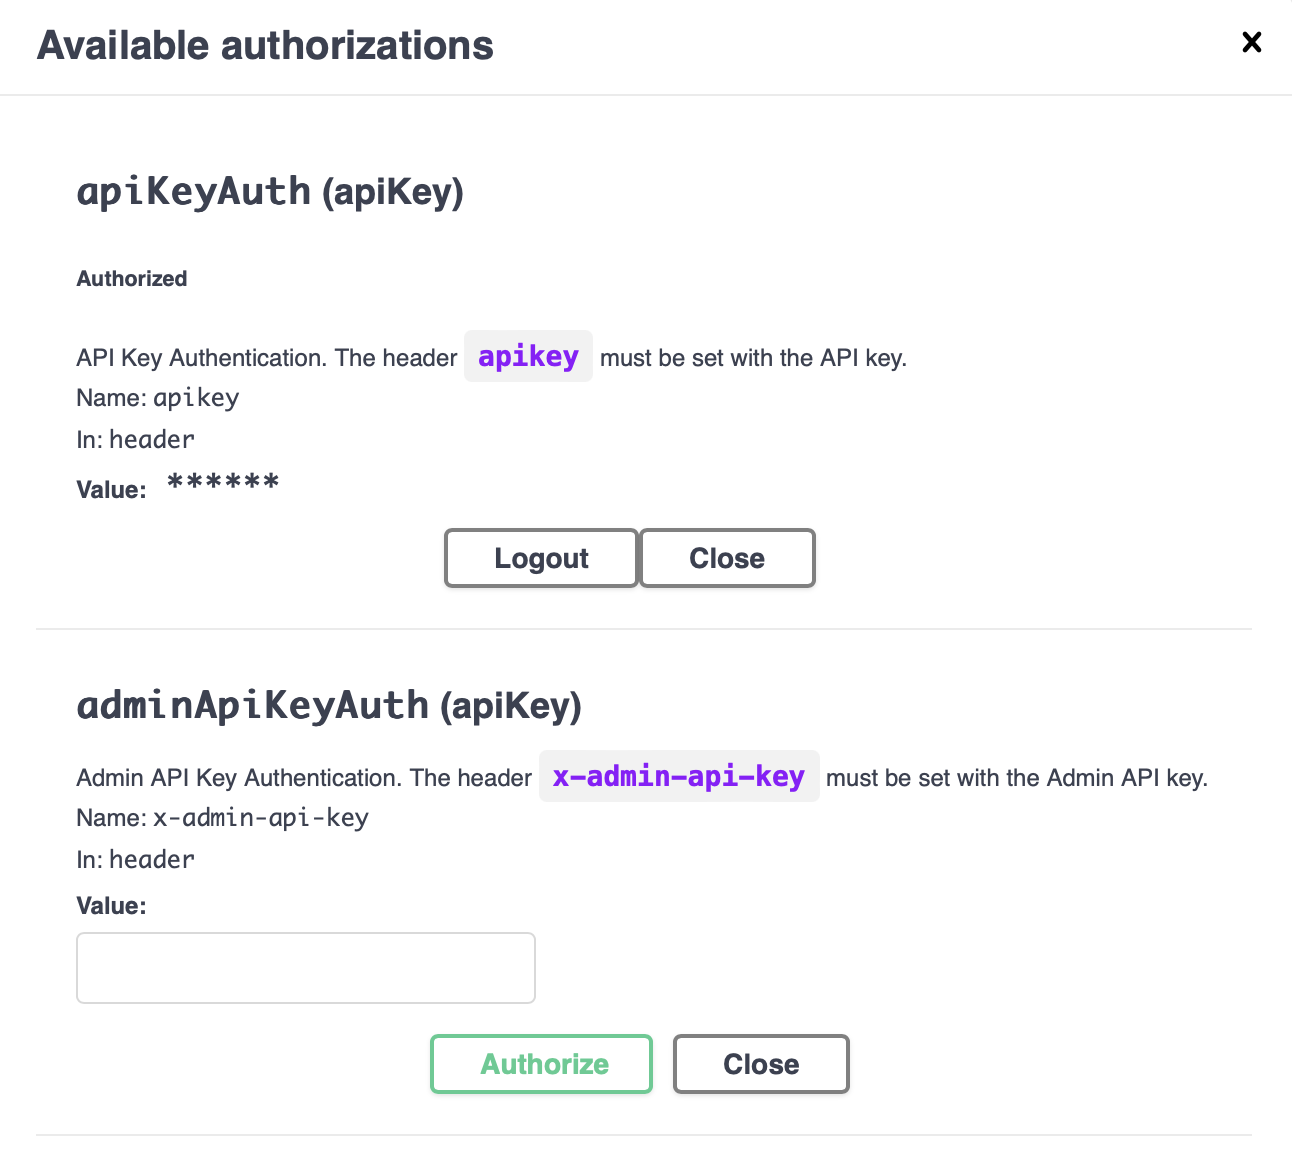
\includegraphics[keepaspectratio]{section2/swagger-ui-apikey-modal.png}}

}

\caption{Swagger UI Apikey Modal}

\end{figure}%

You can close that modal window and try your first request, click to
expand the \texttt{GET\ /connections} endpoint and click
\texttt{Try\ it\ out} button, that will enable the text inputs for any
available parameters, for now, all three parameters should be blank
(\texttt{offet}, \texttt{limit}, \texttt{thid}).

Finally, just click the \texttt{Execute} button to actually perform the
request. This should return something like this:

\begin{Shaded}
\begin{Highlighting}[]
\FunctionTok{\{} \DataTypeTok{"contents"}\FunctionTok{:} \OtherTok{[]}\FunctionTok{,} \DataTypeTok{"kind"}\FunctionTok{:} \StringTok{"ConnectionsPage"}\FunctionTok{,} \DataTypeTok{"self"}\FunctionTok{:} \StringTok{""}\FunctionTok{,} \DataTypeTok{"pageOf"}\FunctionTok{:} \StringTok{""} \FunctionTok{\}}
\end{Highlighting}
\end{Shaded}

Congratulations! you have connected to the API and asked for a list of
\texttt{connections}, right now there are no connections so the empty
array you get back is correct.

\begin{tcolorbox}[enhanced jigsaw, opacitybacktitle=0.6, coltitle=black, opacityback=0, title=\textcolor{quarto-callout-note-color}{\faInfo}\hspace{0.5em}{Note}, colback=white, breakable, toprule=.15mm, leftrule=.75mm, bottomrule=.15mm, toptitle=1mm, bottomtitle=1mm, colframe=quarto-callout-note-color-frame, colbacktitle=quarto-callout-note-color!10!white, left=2mm, titlerule=0mm, arc=.35mm, rightrule=.15mm]

You can use Swagger UI to copy \texttt{curl} commands that you can paste
in your terminal, this will run exactly the same API request. For
example:

\begin{Shaded}
\begin{Highlighting}[]
\ExtensionTok{curl} \AttributeTok{{-}X} \StringTok{\textquotesingle{}GET\textquotesingle{}} \DataTypeTok{\textbackslash{}}
  \StringTok{\textquotesingle{}http://localhost/cloud{-}agent/connections\textquotesingle{}} \DataTypeTok{\textbackslash{}}
  \AttributeTok{{-}H} \StringTok{\textquotesingle{}accept: application/json\textquotesingle{}} \DataTypeTok{\textbackslash{}}
  \AttributeTok{{-}H} \StringTok{\textquotesingle{}apikey: test\textquotesingle{}}
\DataTypeTok{\{}\StringTok{"contents"}\DataTypeTok{:[]}\OperatorTok{,}\StringTok{"kind"}\DataTypeTok{:}\StringTok{"ConnectionsPage"}\OperatorTok{,}\StringTok{"self"}\DataTypeTok{:}\StringTok{""}\OperatorTok{,}\StringTok{"pageOf"}\DataTypeTok{:}\StringTok{""}\DataTypeTok{\}}
\end{Highlighting}
\end{Shaded}

\end{tcolorbox}

\section{Postman}\label{postman}

\texttt{Postman}is perhaps the most popular API tool among developers,
it allow us to easily interact and debug API endpoints but has many
killer feature like enabling teams to share and work together on the
same API, run automated tests, automatically renew tokens, keeps the
state of your interactions with the API, copy code snippets to make API
calls over many languages, etc. So it's really a better overall option
versus the Swagger UI interface or just directly using \texttt{curl}.

The big time saver for us is that because it supports OAS, we can easily
import the whole API definition. So, let's try it:

\begin{enumerate}
\def\labelenumi{\arabic{enumi}.}
\tightlist
\item
  If you don't already have it, first you should
  \href{https://www.postman.com/downloads/}{Download Postman} and
  \href{https://identity.getpostman.com/signup?continue=https\%3A\%2F\%2Fgo.postman.co\%2Fhome}{Sign
  Up} for a free account.
\item
  Head to the
  \href{https://hyperledger.github.io/identus-docs/agent-api/}{API docs}
  and click the Download button, or copy this direct link
  \texttt{https://hyperledger.github.io/identus-docs/redocusaurus/plugin-redoc-0.yaml}
\item
  Inside Postman, go to \texttt{File\ -\textgreater{}\ Import} and
  either drag \& drop your yaml file if you downloaded it or paste the
  URL in the box, this will auto advance to the next step.
\item
  On the ``How to import'' step select ``OpenAPI 3.0 with a Postman
  Collection'' and click import.
\end{enumerate}

If everything goes correctly, you should see ``Identus Cloud Agent API
Reference'' in your collections.

\section{Tutorials}\label{tutorials}

The official documentation contains a
\href{https://hyperledger.github.io/identus-docs/tutorials/}{tutorials}
section with detailed walkthroughs for each of the most important
interactions like connecting to another peer, managing DIDs, managing VC
Schemas, issuing a VC, etc. We highly encourage you to follow those and
get familiar with the API, this will come in very handy very soon when
we start building our own example app.

\part{Section III - Building}

\chapter{Example Project}\label{example-project}

\section{Overview - Airline Ticket
Wallet}\label{overview---airline-ticket-wallet}

One of the best ways to learn and understand a software platform is to
build something with it. In the following chapters, we will build an
example application showing how to use Identus to issue and verify
airline tickets.

Users will be able to purchase a flight, and receive a Verifiable
Credential representing a ticket and seat assignment. Travelers will be
able to present their ticket to Airport Security when requested, and in
turn, the security officer will be able to verify the ticket's
authenticity.

We will use the Identus Cloud Agent, plus the Typescript SDK in our
examples, however the same functionality and source is available in the
native language of each Edge Agent SDK; Swift for iOS/Mac and Kotlin for
Android. Please see the book's Github page for the complete source code
and follow along in your language of choice.

\section{Prerequisites}\label{prerequisites}

To follow along with the book, please make sure you have a working Cloud
Agent development environment, as described in the
\href{../section2/installation-local.md}{Section 2}.

\section{Roles}\label{roles}

\subsection{Issuer: Airline}\label{issuer-airline}

\subsection{Holder: Traveler}\label{holder-traveler}

\subsection{Verifier: Airport Security
Officer}\label{verifier-airport-security-officer}

\chapter{Wallets}\label{wallets}

\section{Overview}\label{overview-1}

Wallets are an essential component on every Self-Sovereign Identity
interaction, and as you might have guessed, just like in the physical
world where a wallet holds your identifiers (IDs), a digital SSI
wallet's function is to store and manage Decentralized Identifiers
(DIDs), Verifiable Credentials (VCs), cryptographic keys, and other
related assets.

Since many SSI frameworks rely on a Blockchain to publish DIDs, there is
a common misconception that SSI wallets work in a similar way. Although
both SSI and Blockchain wallets require a \texttt{seed\ phrase} built
from a random set of \texttt{mnemonics}, thats where the overlap ends,
because the balance and history of a Blockchain wallet can be restored
from the ledger itself as opposed to an SSI wallet, where all the stored
information exists only on the device and needs to be manually backed up
and restored.

In essence, a wallet in SSI is piece of software that allows users to
store, manage, and present proof of their digital identities and
credentials. It acts as a repository for digital assets required to
fulfill every SSI interaction, ensuring that users and entities have
complete control over their data. In the case of Identus, the
\href{https://github.com/hyperledger/identus-edge-agent-sdk-ts}{Edge
Agent SDK} provides all the abstractions needed to operate a wallet by
an individual on a browser or mobile app, and the
\href{https://github.com/hyperledger/identus-cloud-agent}{Cloud Agent},
provides a \texttt{REST\ API} to operate a wallet in the cloud, either
to itself (single tenant) or for third-parties (multi tenant) as a
custodial wallet.

\section{Edge Agent SDK in Identus}\label{edge-agent-sdk-in-identus}

Identus provides it's wallet interface through the Edge Agent SDKs,
available in 3 flavors:

\begin{itemize}
\tightlist
\item
  \href{https://github.com/hyperledger/identus-edge-agent-sdk-ts}{TypeScript}
  for Web and Node apps.
\item
  \href{https://github.com/hyperledger/identus-edge-agent-sdk-swift}{Swift}
  for iOS and Mac.
\item
  \href{https://github.com/hyperledger/identus-edge-agent-sdk-kmp}{Kotlin}
  for Android and JVM.
\end{itemize}

Each of the flavors provide the same building block implementations:

\begin{itemize}
\tightlist
\item
  Apollo: Provides a suite of necessary cryptographic operations.
\item
  Castor: Provides a suite of operations to create, manage and resolve
  decentralized identifiers.
\item
  Pollux: Provides a suite of operations for
  handling~\href{https://github.com/hyperledger/identus-docs/blob/master/documentation/docs/concepts/glossary.md\#verifiable-credentials}{verifiable
  credentials}.
\item
  Mercury: Provides a suite of operations for handling DIDComm V2
  messages.
\item
  Pluto: Provides an interface for storage operations in a portable,
  storage-agnostic manner.
\item
  Agent: A component using all other building blocks, provides basic
  edge agent capabilities, including implementing DIDComm V2 protocols.
\end{itemize}

And all of them abstract the usage of each building block through the
Agent component.

Most of the time you will be operating the wallet trough the Agent
interface unless you require to directly call lower level building block
API, for example, you may require to send a custom DIDCOMM message
payload format which is not directly supported via the Agent building
block, you can still use Mercury directly to achieve that. This approach
gives you a simple to use interface trough the Agent but also the
flexibility and control that comes with also providing access to the
lower level APIs. We highly encourage to dig inside each of the building
blocks and study how the Agent is using them, this will come handy when
you need to add custom features to your own software.

There is one building block that is \emph{not} implemented and only
provided as an interface, this is Pluto, the storage layer for DIDs,
VCs, messages, keys, etc. Identus does not have an opinion on how you
should store and retrieve the contents of the wallet, so it's your job
to implement this part according to your needs. Fortunately, there is a
community project providing one implementation called
\href{https://github.com/atala-community-projects/pluto-encrypted}{Pluto
Encrypted}, this project provides 3 different storage engines: InMemory,
IndexDB, LevelDB. As the name suggest, Pluto Encrypted provides full
Pluto compatibility plus handles encryption and decryption of the wallet
contents, this is very important due to the fact that the wallet stores
your DIDs (private keys), VCs, messages and a lot of sensitive
information. If you are starting out we highly recommend you to use this
implementation before attempting to role your own, it's a great starting
place that you can extend and customize to your needs.

\section{Custodial Wallets}\label{custodial-wallets}

In an ideal world, everyone should be willing and able to manage their
own identity wallets, this is one of the main characteristics of truly
Self-Sovereign ecosystem. In practice, there are many good reasons why
an identity wallet would be better managed by a service. Such is the
case for companies and entities or even individuals that don't want to
deal with the responsibility and risk of self-managing their wallets.
For this use case Identus provides the concept of Custodial Wallets.
What this really means is that an identity wallet can be managed by the
Cloud Agent and used over a REST API. For this particular use case, the
Cloud Agent supports a multi-tenant mode in order to onboard and serve
multiple identity wallets on the same running instance. We will explain
the setup in detail over the production installation section, for now
the key insight is that when you access your identity wallet through a
Cloud Agent, you are really trusting the storage and management of the
private keys of your identity to that service.

\chapter{DIDs and DID Documents}\label{dids-and-did-documents}

\section{Overview}\label{overview-2}

A \textbf{DID Document} (\emph{Decentralized Identifier Document}) is a
JSON-LD (\emph{JavaScript Object Notation for Linked Data}) structure
which describes a Subject. This can represent the identity of a person,
a thing, or a relationship between one or many entities. Contained in
the document is information which can verify that identity without
relying on a centralized authority.

A \textbf{DID} (\emph{Decentralized Identifier}) is the canonical
representation of a DIDDocument; a portable, compact hash, which can be
passed around easily or stored to a database or blockchain. A DID can be
\emph{resolved}, revealing the full, parsable JSON encoded DIDDocument.

The spec for a \texttt{did:prism} DIDDocument can be found
\href{https://github.com/input-output-hk/prism-did-method-spec/blob/main/w3c-spec/PRISM-method.md\#did-documents}{here}.

An Example DID:
\texttt{did:prism:4a5b5cf0a513e83b598bbea25cd6196746747f065246f1d3743344b4b81b5a74:Cr4BCrsBElsKBmF1dGgwMRJRCglzZWNwMjU2azESBHRlc3QaOmtleTE6Ly8wMjM5MmYxNjc4NmNlNmQ0NzJlOGViNzA4ZWRjMmE3OTFmZGMxNzNkNjVkNTBhODNhMTk3N2I5ZmIwMmU0MjQSWwoGYXV0aDAyElEKCXNlY3AyNTZrMRIEdGVzdBo6a2V5MjovLzAyMzkyZjE2Nzg2Y2U2ZDQ3MmU4ZWI3MDhlZGMyYTc5MWZkYzE3M2Q2NWQ1MGE4M2ExOTc3YjlmYjAyZTQyNA}

Let's break down the format of this example DID:

\begin{itemize}
\tightlist
\item
  \texttt{did:prism:} The prefix of the DID
\item
  \texttt{4a5b5cf0a513e83b598bbea25cd6196746747f065246f1d3743344b4b81b5a74}:
  The DID identifier. This can be anything, as long as it is unique to
  the DID Document it is describing, and means something to your
  application.
\item
  \texttt{Cr4BCrsBElsKBmF1dGgwMRJRCglzZWNwMjU...}: The DID Document
  itself, encoded in base58
\end{itemize}

An Example DIDDocument:

\begin{Shaded}
\begin{Highlighting}[]
\FunctionTok{\{}
  \DataTypeTok{"@context"}\FunctionTok{:} \OtherTok{[}
      \StringTok{"https://www.w3.org/ns/did/v1"}\OtherTok{,}
      \StringTok{"https://w3id.org/security/suites/jws{-}2020/v1"}\OtherTok{,}
      \StringTok{"https://didcomm.org/messaging/contexts/v2"}\OtherTok{,}
      \StringTok{"https://identity.foundation/.well{-}known/did{-}configuration/v1"}
    \OtherTok{]}\FunctionTok{,}
  \DataTypeTok{"id"}\FunctionTok{:} \StringTok{"did:prism:123456789abcdefghi"}\FunctionTok{,}
  \DataTypeTok{"controller"}\FunctionTok{:} \StringTok{"did:example:bcehfew7h32f32h7af3"}\FunctionTok{,}
  \DataTypeTok{"verificationMethod"}\FunctionTok{:} \OtherTok{[}\FunctionTok{\{}
    \DataTypeTok{"id"}\FunctionTok{:} \StringTok{"did:prism:123456789abcdefghi\#key{-}1"}\FunctionTok{,}
    \DataTypeTok{"type"}\FunctionTok{:} \StringTok{"JsonWebKey2020"}\FunctionTok{,}
    \DataTypeTok{"controller"}\FunctionTok{:} \OtherTok{[}\StringTok{"did:prism:123456789abcdefghi"}\OtherTok{]}\FunctionTok{,}
    \DataTypeTok{"publicKeyJwk"}\FunctionTok{:} \FunctionTok{\{}
      \DataTypeTok{"kty"}\FunctionTok{:} \StringTok{"OKP"}\FunctionTok{,}
      \DataTypeTok{"crv"}\FunctionTok{:} \StringTok{"Ed25519"}\FunctionTok{,}
      \DataTypeTok{"x"}\FunctionTok{:} \StringTok{"VCpo2LMLhn6iWku8MKvSLg2ZAoC{-}nlOyPVQaO3FxVeQ"}
    \FunctionTok{\}}
  \FunctionTok{\}}\OtherTok{]}\FunctionTok{,}
  \DataTypeTok{"authentication"}\FunctionTok{:} \OtherTok{[}\StringTok{"did:prism:123456789abcdefghi\#key{-}1"}\OtherTok{]}\FunctionTok{,}
  \DataTypeTok{"assertionMethod"}\FunctionTok{:} \OtherTok{[}\StringTok{"did:prism:123456789abcdefghi\#key{-}1"}\OtherTok{]}\FunctionTok{,}
  \DataTypeTok{"keyAgreement"}\FunctionTok{:} \OtherTok{[} \StringTok{"did:prism:123456789abcdefghi\#key{-}1"}\OtherTok{]}\FunctionTok{,}
  \DataTypeTok{"service"}\FunctionTok{:} \OtherTok{[}\FunctionTok{\{}
    \DataTypeTok{"id"}\FunctionTok{:} \StringTok{"did:prism:123456789abcdefghi\#messaging"}\FunctionTok{,}
    \DataTypeTok{"type"}\FunctionTok{:} \StringTok{"DIDCommMessaging"}\FunctionTok{,}
    \DataTypeTok{"serviceEndpoint"}\FunctionTok{:} \StringTok{"https://example.com/endpoint"}
  \FunctionTok{\}}\OtherTok{]}
\FunctionTok{\}}
\end{Highlighting}
\end{Shaded}

Let's look at the components of a DID Document:

\begin{itemize}
\tightlist
\item
  \textbf{\texttt{id}}: The DID of the Subject described by the
  DIDDocument
\item
  \textbf{\texttt{@context}}: This is an array of specifications used in
  this DIDDocument. The first element is usually
  \url{https://www.w3.org/ns/did/v1} but any other common definitions
  are
  \href{https://w3id.org/security/suites/jws-2020/v1}{JSONWebSignature}
  or \href{https://didcomm.org/messaging/contexts/v2}{DIDComm2
  Messaging} protocols.
\item
  \textbf{\texttt{controller}}: An array of DIDs that are allowed to
  mutate the DIDDocument
\item
  \textbf{\texttt{verificationMethod}}: An array of information which
  can be used to verify the identity of the Subject.

  \begin{itemize}
  \tightlist
  \item
    \texttt{id}: The DID of the Subject
  \item
    \texttt{controller}: The DID of the Subject (author's note: When
    could this be different than id?)
  \item
    \href{https://www.w3.org/TR/did-core/\#dfn-publickeyjwk}{publicKeyJwk}
    or
    \href{https://www.w3.org/TR/did-core/\#dfn-publickeymultibase}{publicKeyMultibase}:

    \begin{itemize}
    \tightlist
    \item
      \texttt{publicKeyJwk}: A JSON Web Key (JWK) representation of the
      Subject's Public Key
    \item
      \texttt{publicKeyMultibase}: An encoded public key using
      \href{https://www.ietf.org/archive/id/draft-multiformats-multibase-08.html}{Multibase}
      encoding
    \end{itemize}
  \item
    \texttt{type}: The type of
    \href{https://www.w3.org/TR/did-core/\#dfn-verification-method}{Verification
    Method}, ie
    \href{https://www.w3.org/community/reports/credentials/CG-FINAL-di-eddsa-2020-20220724/\#ed25519verificationkey2020}{\texttt{Ed25519VerificationKey2020}}
    or
    \href{https://www.w3.org/community/reports/credentials/CG-FINAL-lds-jws2020-20220721/\#json-web-key-2020}{JsonWebKey2020}
  \end{itemize}
\item
  \textbf{Authentication Methods}:

  \begin{itemize}
  \tightlist
  \item
    \texttt{authentication}, \texttt{assertionMethod},
    \texttt{keyAgreement}: Arrays of locations in the Subject DID,
    referenced in a DID + anchor format
    (\texttt{did:prism:1234\#authentication0})
  \item
    *Author's note - Specify these in a more concrete way
  \end{itemize}
\item
  \textbf{\texttt{service}}: An array of advertised methods of
  interacting with the Subject. These could be API endpoints for
  messaging or file storage systems, but any remote service can be added
  to add value to the DID.
\end{itemize}

An non-exhaustive example of a \texttt{did:prism} DIDDocument can be
found
\href{https://github.com/input-output-hk/prism-did-method-spec/blob/main/w3c-spec/PRISM-method.md\#example-did-document-json-ld}{here}.

\section{Resolvers}\label{resolvers}

A resolver is a service that can resolve a DID to a DIDDocument. There
are PRISM specific resolvers built into Identus SDKs, or you can also
run your own resolver service.

Some third-party PRISM resolvers:

\begin{itemize}
\tightlist
\item
  \href{https://analytics.blocktrust.dev/resolve}{Blocktrust Resolver}
\item
  \href{https://neoprism.patlo.dev/resolver}{NeoPrism Resolver}
\end{itemize}

\section{Controllers}\label{controllers}

\textbf{Controllers} are entities that can mutate the DIDDocument.
Controllers are specified in the DIDDocument as an array of DIDs so they
can be a person, thing, or organization.

Remember that DIDs can all be resolved to DIDDocuments, and each
DIDDocument can point to people, things, machines, or services. Every
mention of a DID can potentially be a chain of references to other
services, or endpoints. There is plenty of room to be creative with this
relationship graph.

\chapter{Connections}\label{connections}

\section{Overview}\label{overview-3}

Now that we have a better understanding of Wallets and DIDs, it's time
to embark on our first interaction. In this chapter we are going to
explore conceptually what a Connection means in SSI, take a deep dive
into DID Peers, explain how they work and why they are needed for secure
connections, dissect Out of Band invites and finally hands on example
code to achieve connecting edge client to an agent.

Before we move forward we highly recommend to at least read the basic
\href{https://hyperledger.github.io/identus-docs/tutorials/connections/connection}{Connection
tutorial} on the official
\href{https://hyperledger.github.io/identus-docs/}{Identus
documentation}.

\section{Connections in Self-Sovereign
Identity}\label{connections-in-self-sovereign-identity}

Connections are fundamental to establishing \emph{trusted interactions}
between peers. They enable secure and verifiable communication, allowing
entities to exchange credentials and proofs in a decentralized manner.
This relationship is established using a specific decentralized
identifier standard (\textbf{Peer DID}) and is governed by a protocol
(\textbf{DIDComm}) that ensure the authenticity, integrity, and privacy
of the interactions between the connected parties.

There are three roles in an SSI connection:

\begin{itemize}
\tightlist
\item
  \textbf{Inviter}: The entity that initiates the connection by sending
  an invitation.
\item
  \textbf{Invitee}: The entity that receives the invitation and responds
  with a connection request.
\item
  \textbf{Mediator}: An intermediary that facilitates message delivery
  between entities, especially when one or both parties may not always
  be online.
\end{itemize}

\begin{tcolorbox}[enhanced jigsaw, opacitybacktitle=0.6, coltitle=black, opacityback=0, title=\textcolor{quarto-callout-note-color}{\faInfo}\hspace{0.5em}{Note}, colback=white, breakable, toprule=.15mm, leftrule=.75mm, bottomrule=.15mm, toptitle=1mm, bottomtitle=1mm, colframe=quarto-callout-note-color-frame, colbacktitle=quarto-callout-note-color!10!white, left=2mm, titlerule=0mm, arc=.35mm, rightrule=.15mm]

We will cover \href{./section4/mediator.html}{mediators} in detail later
on. For now what you need to understand is that they are used as a
service to relay messages between peers, they will store messages and
deliver them whenever a peer comes back online, connects to the mediator
and fetches their messages.

\end{tcolorbox}

\section{PeerDIDs}\label{peerdids}

They are a special kind of decentralized identifier with some unique
properties that allow them to be perfect for use in order to establish
private and secure communications between peers.

DID Documents such as PrismDIDs are meant to be publicly available and
resolvable by arbitrary parties, therefor storing them in a VDR such as
Cardano blockchain is an excellent way to achieve this requirement in a
reliable way.

However, when Alice and Bob want to interact with each other, only two
parties care about the details of that connection: Alice and Bob.
Instead of arbitrary parties needing to resolve their DIDs, only Alice
and Bob do. Thus, PeerDIDs essentially describe a key-pair to encrypt
and sign data to and from Alice and Bob, routed trough their preferred
mediators, e.g.~When Alice accepts an invite from Bob and they engage
the connection protocol, Alice generates a PeerDID that allows her to
encrypt and sign data routed trough Bob's mediator (mediator Y) that
only Bob can decrypt, and vice versa, Bob will generate a PeerDID that
allows him to encrypt and sign data routed trough Alice's preferred
mediator (mediator X) that only Alice can decrypt.

The key benefits of PeerDIDs are:

\begin{enumerate}
\def\labelenumi{\arabic{enumi}.}
\tightlist
\item
  Decentralized by nature.
\item
  No transaction cost on blockchain.
\item
  Private (only the concerned parties know about them).
\item
  Reusable without any reliance on the internet, with no degradation of
  trust. (adheres to the principles of
  \href{https://www.inkandswitch.com/local-first/}{local-first} and
  \href{https://offlinefirst.org}{offline-first})
\end{enumerate}

Lets resolve a PeerDID, we call resolve to the unpacking and parsing of
a DID in order to read its content and use the DID for the interactions
that we need to achieve. For this example we will resolve a PeerDID from
\href{https://sandbox-mediator.atalaprism.io}{Atala's mediator sandbox}.

\begin{Shaded}
\begin{Highlighting}[]
\ExtensionTok{curl}\NormalTok{ https://sandbox{-}mediator.atalaprism.io/did}

\ExtensionTok{did:peer:2.Ez6LSghwSE437wnDE1pt3X6hVDUQzSjsHzinpX3XFvMjRAm7y.Vz6Mkhh1e5CEYYq6JBUcTZ6Cp2ranCWRrv7Yax3Le4N59R6dd.SeyJ0IjoiZG0iLCJzIjp7InVyaSI6Imh0dHBzOi8vc2FuZGJveC1tZWRpYXRvci5hdGFsYXByaXNtLmlvIiwiYSI6WyJkaWRjb21tL3YyIl19fQ.SeyJ0IjoiZG0iLCJzIjp7InVyaSI6IndzczovL3NhbmRib3gtbWVkaWF0b3IuYXRhbGFwcmlzbS5pby93cyIsImEiOlsiZGlkY29tbS92MiJdfX0}
\end{Highlighting}
\end{Shaded}

We can see that the mediator returned a PeerDID when we send a
\texttt{GET} request to the \texttt{/did} endpoint. In order to resolve
this DID we can use an \href{https://dev.uniresolver.io}{Universal
Resolver} website for this example:

\begin{Shaded}
\begin{Highlighting}[]
\ExtensionTok{curl}\NormalTok{ https://dev.uniresolver.io/1.0/identifiers/did:peer:2.Ez6LSghwSE437wnDE1pt3X6hVDUQzSjsHzinpX3XFvMjRAm7y.Vz6Mkhh1e5CEYYq6JBUcTZ6Cp2ranCWRrv7Yax3Le4N59R6dd.SeyJ0IjoiZG0iLCJzIjp7InVyaSI6Imh0dHBzOi8vc2FuZGJveC1tZWRpYXRvci5hdGFsYXByaXNtLmlvIiwiYSI6WyJkaWRjb21tL3YyIl19fQ.SeyJ0IjoiZG0iLCJzIjp7InVyaSI6IndzczovL3NhbmRib3gtbWVkaWF0b3IuYXRhbGFwcmlzbS5pby93cyIsImEiOlsiZGlkY29tbS92MiJdfX0}
\end{Highlighting}
\end{Shaded}

\begin{Shaded}
\begin{Highlighting}[]
\FunctionTok{\{}
  \DataTypeTok{"@context"}\FunctionTok{:} \StringTok{"https://w3id.org/did{-}resolution/v1"}\FunctionTok{,}
  \DataTypeTok{"didDocument"}\FunctionTok{:} \FunctionTok{\{}
    \DataTypeTok{"@context"}\FunctionTok{:} \OtherTok{[}
      \StringTok{"https://www.w3.org/ns/did/v1"}\OtherTok{,}
      \StringTok{"https://w3id.org/security/multikey/v1"}\OtherTok{,}
      \FunctionTok{\{}
        \DataTypeTok{"@base"}\FunctionTok{:} \StringTok{"did:peer:2.Ez6LSghwSE437wnDE1pt3X6hVDUQzSjsHzinpX3XFvMjRAm7y.Vz6Mkhh1e5CEYYq6JBUcTZ6Cp2ranCWRrv7Yax3Le4N59R6dd.SeyJ0IjoiZG0iLCJzIjp7InVyaSI6Imh0dHBzOi8vc2FuZGJveC1tZWRpYXRvci5hdGFsYXByaXNtLmlvIiwiYSI6WyJkaWRjb21tL3YyIl19fQ.SeyJ0IjoiZG0iLCJzIjp7InVyaSI6IndzczovL3NhbmRib3gtbWVkaWF0b3IuYXRhbGFwcmlzbS5pby93cyIsImEiOlsiZGlkY29tbS92MiJdfX0"}
      \FunctionTok{\}}
    \OtherTok{]}\FunctionTok{,}
    \DataTypeTok{"id"}\FunctionTok{:} \StringTok{"did:peer:2.Ez6LSghwSE437wnDE1pt3X6hVDUQzSjsHzinpX3XFvMjRAm7y.Vz6Mkhh1e5CEYYq6JBUcTZ6Cp2ranCWRrv7Yax3Le4N59R6dd.SeyJ0IjoiZG0iLCJzIjp7InVyaSI6Imh0dHBzOi8vc2FuZGJveC1tZWRpYXRvci5hdGFsYXByaXNtLmlvIiwiYSI6WyJkaWRjb21tL3YyIl19fQ.SeyJ0IjoiZG0iLCJzIjp7InVyaSI6IndzczovL3NhbmRib3gtbWVkaWF0b3IuYXRhbGFwcmlzbS5pby93cyIsImEiOlsiZGlkY29tbS92MiJdfX0"}\FunctionTok{,}
    \DataTypeTok{"verificationMethod"}\FunctionTok{:} \OtherTok{[}
      \FunctionTok{\{}
        \DataTypeTok{"id"}\FunctionTok{:} \StringTok{"\#key{-}2"}\FunctionTok{,}
        \DataTypeTok{"type"}\FunctionTok{:} \StringTok{"Multikey"}\FunctionTok{,}
        \DataTypeTok{"controller"}\FunctionTok{:} \StringTok{"did:peer:2.Ez6LSghwSE437wnDE1pt3X6hVDUQzSjsHzinpX3XFvMjRAm7y.Vz6Mkhh1e5CEYYq6JBUcTZ6Cp2ranCWRrv7Yax3Le4N59R6dd.SeyJ0IjoiZG0iLCJzIjp7InVyaSI6Imh0dHBzOi8vc2FuZGJveC1tZWRpYXRvci5hdGFsYXByaXNtLmlvIiwiYSI6WyJkaWRjb21tL3YyIl19fQ.SeyJ0IjoiZG0iLCJzIjp7InVyaSI6IndzczovL3NhbmRib3gtbWVkaWF0b3IuYXRhbGFwcmlzbS5pby93cyIsImEiOlsiZGlkY29tbS92MiJdfX0"}\FunctionTok{,}
        \DataTypeTok{"publicKeyMultibase"}\FunctionTok{:} \StringTok{"z6Mkhh1e5CEYYq6JBUcTZ6Cp2ranCWRrv7Yax3Le4N59R6dd"}
      \FunctionTok{\}}\OtherTok{,}
      \FunctionTok{\{}
        \DataTypeTok{"id"}\FunctionTok{:} \StringTok{"\#key{-}1"}\FunctionTok{,}
        \DataTypeTok{"type"}\FunctionTok{:} \StringTok{"Multikey"}\FunctionTok{,}
        \DataTypeTok{"controller"}\FunctionTok{:} \StringTok{"did:peer:2.Ez6LSghwSE437wnDE1pt3X6hVDUQzSjsHzinpX3XFvMjRAm7y.Vz6Mkhh1e5CEYYq6JBUcTZ6Cp2ranCWRrv7Yax3Le4N59R6dd.SeyJ0IjoiZG0iLCJzIjp7InVyaSI6Imh0dHBzOi8vc2FuZGJveC1tZWRpYXRvci5hdGFsYXByaXNtLmlvIiwiYSI6WyJkaWRjb21tL3YyIl19fQ.SeyJ0IjoiZG0iLCJzIjp7InVyaSI6IndzczovL3NhbmRib3gtbWVkaWF0b3IuYXRhbGFwcmlzbS5pby93cyIsImEiOlsiZGlkY29tbS92MiJdfX0"}\FunctionTok{,}
        \DataTypeTok{"publicKeyMultibase"}\FunctionTok{:} \StringTok{"z6LSghwSE437wnDE1pt3X6hVDUQzSjsHzinpX3XFvMjRAm7y"}
      \FunctionTok{\}}
    \OtherTok{]}\FunctionTok{,}
    \DataTypeTok{"keyAgreement"}\FunctionTok{:} \OtherTok{[}
      \StringTok{"\#key{-}1"}
    \OtherTok{]}\FunctionTok{,}
    \DataTypeTok{"authentication"}\FunctionTok{:} \OtherTok{[}
      \StringTok{"\#key{-}2"}
    \OtherTok{]}\FunctionTok{,}
    \DataTypeTok{"assertionMethod"}\FunctionTok{:} \OtherTok{[}
      \StringTok{"\#key{-}2"}
    \OtherTok{]}\FunctionTok{,}
    \DataTypeTok{"service"}\FunctionTok{:} \OtherTok{[}
      \FunctionTok{\{}
        \DataTypeTok{"serviceEndpoint"}\FunctionTok{:} \FunctionTok{\{}
          \DataTypeTok{"uri"}\FunctionTok{:} \StringTok{"https://sandbox{-}mediator.atalaprism.io"}\FunctionTok{,}
          \DataTypeTok{"accept"}\FunctionTok{:} \OtherTok{[}
            \StringTok{"didcomm/v2"}
          \OtherTok{]}
        \FunctionTok{\},}
        \DataTypeTok{"type"}\FunctionTok{:} \StringTok{"DIDCommMessaging"}\FunctionTok{,}
        \DataTypeTok{"id"}\FunctionTok{:} \StringTok{"\#service"}
      \FunctionTok{\}}\OtherTok{,}
      \FunctionTok{\{}
        \DataTypeTok{"serviceEndpoint"}\FunctionTok{:} \FunctionTok{\{}
          \DataTypeTok{"uri"}\FunctionTok{:} \StringTok{"wss://sandbox{-}mediator.atalaprism.io/ws"}\FunctionTok{,}
          \DataTypeTok{"accept"}\FunctionTok{:} \OtherTok{[}
            \StringTok{"didcomm/v2"}
          \OtherTok{]}
        \FunctionTok{\},}
        \DataTypeTok{"type"}\FunctionTok{:} \StringTok{"DIDCommMessaging"}\FunctionTok{,}
        \DataTypeTok{"id"}\FunctionTok{:} \StringTok{"\#service{-}1"}
      \FunctionTok{\}}
    \OtherTok{]}
  \FunctionTok{\},}
  \DataTypeTok{"didResolutionMetadata"}\FunctionTok{:} \FunctionTok{\{}
    \DataTypeTok{"contentType"}\FunctionTok{:} \StringTok{"application/did+ld+json"}\FunctionTok{,}
    \DataTypeTok{"pattern"}\FunctionTok{:} \StringTok{"\^{}(did:peer:.+)$"}\FunctionTok{,}
    \DataTypeTok{"driverUrl"}\FunctionTok{:} \StringTok{"http://uni{-}resolver{-}driver{-}did{-}uport:8081/1.0/identifiers/"}\FunctionTok{,}
    \DataTypeTok{"duration"}\FunctionTok{:} \DecValTok{4}\FunctionTok{,}
    \DataTypeTok{"driverDuration"}\FunctionTok{:} \DecValTok{4}\FunctionTok{,}
    \DataTypeTok{"did"}\FunctionTok{:} \FunctionTok{\{}
      \DataTypeTok{"didString"}\FunctionTok{:} \StringTok{"did:peer:2.Ez6LSghwSE437wnDE1pt3X6hVDUQzSjsHzinpX3XFvMjRAm7y.Vz6Mkhh1e5CEYYq6JBUcTZ6Cp2ranCWRrv7Yax3Le4N59R6dd.SeyJ0IjoiZG0iLCJzIjp7InVyaSI6Imh0dHBzOi8vc2FuZGJveC1tZWRpYXRvci5hdGFsYXByaXNtLmlvIiwiYSI6WyJkaWRjb21tL3YyIl19fQ.SeyJ0IjoiZG0iLCJzIjp7InVyaSI6IndzczovL3NhbmRib3gtbWVkaWF0b3IuYXRhbGFwcmlzbS5pby93cyIsImEiOlsiZGlkY29tbS92MiJdfX0"}\FunctionTok{,}
      \DataTypeTok{"methodSpecificId"}\FunctionTok{:} \StringTok{"2.Ez6LSghwSE437wnDE1pt3X6hVDUQzSjsHzinpX3XFvMjRAm7y.Vz6Mkhh1e5CEYYq6JBUcTZ6Cp2ranCWRrv7Yax3Le4N59R6dd.SeyJ0IjoiZG0iLCJzIjp7InVyaSI6Imh0dHBzOi8vc2FuZGJveC1tZWRpYXRvci5hdGFsYXByaXNtLmlvIiwiYSI6WyJkaWRjb21tL3YyIl19fQ.SeyJ0IjoiZG0iLCJzIjp7InVyaSI6IndzczovL3NhbmRib3gtbWVkaWF0b3IuYXRhbGFwcmlzbS5pby93cyIsImEiOlsiZGlkY29tbS92MiJdfX0"}\FunctionTok{,}
      \DataTypeTok{"method"}\FunctionTok{:} \StringTok{"peer"}
    \FunctionTok{\}}
  \FunctionTok{\},}
  \DataTypeTok{"didDocumentMetadata"}\FunctionTok{:} \FunctionTok{\{\}}
\FunctionTok{\}}
\end{Highlighting}
\end{Shaded}

This is what a PeerDID looks like when resolved, please bear in mind
that the JSON-LD context for \texttt{did-resolution} and extra
\texttt{didResolutionMetadata} entry are added by the resolver and the
actual isolated PeerDID is only what we see inside the
\texttt{didDocument} payload.

In simple terms, a PeerDID is essentially a JSON payload that contains a
set of keys and an optional service endpoints, because this is a
mediator PeerDID, it contains service endpoints for
\texttt{DIDCommMessaging}, in this particular case, you can see it
contains two of them, one over regular \texttt{https} and other trough
\texttt{websockets}.

To go deeper in your understanding of PeerDIDs please refer to the full
\href{https://identity.foundation/peer-did-method-spec}{Peer DID Method
Specification}. In the Hyperledger Identus ecosystem, only PeerDIDs
method 2 are supported at the time of this writing.

\section{Out of Band invites}\label{out-of-band-invites}

Out of Band (OOB) invites are the entry point for some protocols to take
place, they usually are encoded in either a JSON payload or a URL and
are distributed ``out of band'', usually over QR codes, but could be
distributed over any medium (Bluetooth, NFC, etc). They gather all
required information for one peer to start interacting with another and
you can think of them as a way to advertise ``coordinates'' for anyone
that would like to establish an interaction to the inviter.

Following the same example as before, we can see that the sandbox
mediator also delivers an OOB invite in a URL form.

\begin{Shaded}
\begin{Highlighting}[]
\ExtensionTok{https://sandbox{-}mediator.atalaprism.io?\_oob=eyJpZCI6ImExNTY4YzEyLTBjZGMtNDY0Ny05ZGM2LWE1YWFkYTZmODI0NyIsInR5cGUiOiJodHRwczovL2RpZGNvbW0ub3JnL291dC1vZi1iYW5kLzIuMC9pbnZpdGF0aW9uIiwiZnJvbSI6ImRpZDpwZWVyOjIuRXo2TFNnaHdTRTQzN3duREUxcHQzWDZoVkRVUXpTanNIemlucFgzWEZ2TWpSQW03eS5WejZNa2hoMWU1Q0VZWXE2SkJVY1RaNkNwMnJhbkNXUnJ2N1lheDNMZTRONTlSNmRkLlNleUowSWpvaVpHMGlMQ0p6SWpwN0luVnlhU0k2SW1oMGRIQnpPaTh2YzJGdVpHSnZlQzF0WldScFlYUnZjaTVoZEdGc1lYQnlhWE50TG1sdklpd2lZU0k2V3lKa2FXUmpiMjF0TDNZeUlsMTlmUS5TZXlKMElqb2laRzBpTENKeklqcDdJblZ5YVNJNkluZHpjem92TDNOaGJtUmliM2d0YldWa2FXRjBiM0l1WVhSaGJHRndjbWx6YlM1cGJ5OTNjeUlzSW1FaU9sc2laR2xrWTI5dGJTOTJNaUpkZlgwIiwiYm9keSI6eyJnb2FsX2NvZGUiOiJyZXF1ZXN0LW1lZGlhdGUiLCJnb2FsIjoiUmVxdWVzdE1lZGlhdGUiLCJhY2NlcHQiOlsiZGlkY29tbS92MiJdfSwidHlwIjoiYXBwbGljYXRpb24vZGlkY29tbS1wbGFpbitqc29uIn0}
\end{Highlighting}
\end{Shaded}

If we decode the value of the \texttt{\_oob} query variable from
\texttt{base64} we get the \texttt{json} payload

\begin{Shaded}
\begin{Highlighting}[]
\FunctionTok{\{}
  \DataTypeTok{"id"} \FunctionTok{:} \StringTok{"a1568c12{-}0cdc{-}4647{-}9dc6{-}a5aada6f8247"}\FunctionTok{,}
  \DataTypeTok{"type"} \FunctionTok{:} \StringTok{"https://didcomm.org/out{-}of{-}band/2.0/invitation"}\FunctionTok{,}
  \DataTypeTok{"from"} \FunctionTok{:} \StringTok{"did:peer:2.Ez6LSghwSE437wnDE1pt3X6hVDUQzSjsHzinpX3XFvMjRAm7y.Vz6Mkhh1e5CEYYq6JBUcTZ6Cp2ranCWRrv7Yax3Le4N59R6dd.SeyJ0IjoiZG0iLCJzIjp7InVyaSI6Imh0dHBzOi8vc2FuZGJveC1tZWRpYXRvci5hdGFsYXByaXNtLmlvIiwiYSI6WyJkaWRjb21tL3YyIl19fQ.SeyJ0IjoiZG0iLCJzIjp7InVyaSI6IndzczovL3NhbmRib3gtbWVkaWF0b3IuYXRhbGFwcmlzbS5pby93cyIsImEiOlsiZGlkY29tbS92MiJdfX0"}\FunctionTok{,}
  \DataTypeTok{"body"} \FunctionTok{:} \FunctionTok{\{}
    \DataTypeTok{"goal\_code"} \FunctionTok{:} \StringTok{"request{-}mediate"}\FunctionTok{,}
    \DataTypeTok{"goal"} \FunctionTok{:} \StringTok{"RequestMediate"}\FunctionTok{,}
    \DataTypeTok{"accept"} \FunctionTok{:} \OtherTok{[}
      \StringTok{"didcomm/v2"}
    \OtherTok{]}
  \FunctionTok{\},}
  \DataTypeTok{"typ"} \FunctionTok{:} \StringTok{"application/didcomm{-}plain+json"}
\FunctionTok{\}}
\end{Highlighting}
\end{Shaded}

As you can see, an Out of Band invite is really just a way to package a
PeerDID and signaling that it can be used for a particular interaction.
In this case, for a \texttt{RequestMediate} goal over \texttt{DIDComm}.

As a refresher from what we covered, a PeerDID is a way to package a set
of keys and optional service endpoints, and so, \emph{because this an
OOB invite from a mediator}, this invite has everything you need (a
PeerDID and set of service endpoints) to establish this service as your
mediator.

\section{Connecting two peers}\label{connecting-two-peers}

Now, lets issue another kind of Out of Band invite, one from the cloud
agent in order to connect.

The Cloud Agent can generate Out of Band invites, this invite then can
be parsed by another peer (say another Cloud Agent or Edge Client) and
use it to establish a connection, the end result should be a DID Peer on
both sides that allow them to send messages to each other over
\texttt{DIDComm}.

So, our first step is to generate the invite:

\begin{Shaded}
\begin{Highlighting}[]
\ExtensionTok{curl} \AttributeTok{{-}{-}location} \StringTok{\textquotesingle{}http://127.0.0.1:8080/cloud{-}agent/connections\textquotesingle{}} \DataTypeTok{\textbackslash{}}
\NormalTok{{-}{-}header }\StringTok{\textquotesingle{}Content{-}Type: application/json\textquotesingle{}} \DataTypeTok{\textbackslash{}}
\NormalTok{{-}{-}header }\StringTok{\textquotesingle{}Accept: application/json\textquotesingle{}} \DataTypeTok{\textbackslash{}}
\NormalTok{{-}{-}data }\StringTok{\textquotesingle{}\{"label": "test"\}\textquotesingle{}}
\end{Highlighting}
\end{Shaded}

\begin{tcolorbox}[enhanced jigsaw, opacitybacktitle=0.6, coltitle=black, opacityback=0, title=\textcolor{quarto-callout-note-color}{\faInfo}\hspace{0.5em}{Note}, colback=white, breakable, toprule=.15mm, leftrule=.75mm, bottomrule=.15mm, toptitle=1mm, bottomtitle=1mm, colframe=quarto-callout-note-color-frame, colbacktitle=quarto-callout-note-color!10!white, left=2mm, titlerule=0mm, arc=.35mm, rightrule=.15mm]

The only parameter we can change when generating an invite is the
\texttt{label}, this is optional and it is a simple string that you can
use to identify the connection later, a good idea would be to use a
\texttt{uuid} that you generate and manage on your systems, or could be
an alias or the reason for the connection, this is all contextual to the
interaction and use case so in our case we will go with ``test''.

\end{tcolorbox}

The Cloud Agent will respond with a payload that should look like this:

\begin{Shaded}
\begin{Highlighting}[]
\FunctionTok{\{}
    \DataTypeTok{"connectionId"}\FunctionTok{:} \StringTok{"fb36eddd{-}d51e{-}42cf{-}a6fe{-}e76d2e638b70"}\FunctionTok{,}
    \DataTypeTok{"thid"}\FunctionTok{:} \StringTok{"fb36eddd{-}d51e{-}42cf{-}a6fe{-}e76d2e638b70"}\FunctionTok{,}
    \DataTypeTok{"label"}\FunctionTok{:} \StringTok{"test"}\FunctionTok{,}
    \DataTypeTok{"role"}\FunctionTok{:} \StringTok{"Inviter"}\FunctionTok{,}
    \DataTypeTok{"state"}\FunctionTok{:} \StringTok{"InvitationGenerated"}\FunctionTok{,}
    \DataTypeTok{"invitation"}\FunctionTok{:} \FunctionTok{\{}
        \DataTypeTok{"id"}\FunctionTok{:} \StringTok{"fb36eddd{-}d51e{-}42cf{-}a6fe{-}e76d2e638b70"}\FunctionTok{,}
        \DataTypeTok{"type"}\FunctionTok{:} \StringTok{"https://didcomm.org/out{-}of{-}band/2.0/invitation"}\FunctionTok{,}
        \DataTypeTok{"from"}\FunctionTok{:} \StringTok{"did:peer:2.Ez6LSgY6Y67mJ75YCZfZYxYEPQJZs3vaEg2Cc91vppoTA7cpj.Vz6MkpX7H7SNA6ooG5snn2MzgyoRadEZtsjNSL1x7HiiLkqyV.SeyJ0IjoiZG0iLCJzIjp7InVyaSI6Imh0dHA6Ly9ob3N0LmRvY2tlci5pbnRlcm5hbDo4MDgwL2RpZGNvbW0iLCJyIjpbXSwiYSI6WyJkaWRjb21tL3YyIl19fQ"}\FunctionTok{,}
        \DataTypeTok{"invitationUrl"}\FunctionTok{:} \StringTok{"https://my.domain.com/path?\_oob=eyJpZCI6ImZiMzZlZGRkLWQ1MWUtNDJjZi1hNmZlLWU3NmQyZTYzOGI3MCIsInR5cGUiOiJodHRwczovL2RpZGNvbW0ub3JnL291dC1vZi1iYW5kLzIuMC9pbnZpdGF0aW9uIiwiZnJvbSI6ImRpZDpwZWVyOjIuRXo2TFNnWTZZNjdtSjc1WUNaZlpZeFlFUFFKWnMzdmFFZzJDYzkxdnBwb1RBN2Nwai5WejZNa3BYN0g3U05BNm9vRzVzbm4yTXpneW9SYWRFWnRzak5TTDF4N0hpaUxrcXlWLlNleUowSWpvaVpHMGlMQ0p6SWpwN0luVnlhU0k2SW1oMGRIQTZMeTlvYjNOMExtUnZZMnRsY2k1cGJuUmxjbTVoYkRvNE1EZ3dMMlJwWkdOdmJXMGlMQ0p5SWpwYlhTd2lZU0k2V3lKa2FXUmpiMjF0TDNZeUlsMTlmUSIsImJvZHkiOnsiYWNjZXB0IjpbXX19"}
    \FunctionTok{\},}
    \DataTypeTok{"createdAt"}\FunctionTok{:} \StringTok{"2025{-}01{-}04T12:37:37.059649293Z"}\FunctionTok{,}
    \DataTypeTok{"metaRetries"}\FunctionTok{:} \DecValTok{5}\FunctionTok{,}
    \DataTypeTok{"self"}\FunctionTok{:} \StringTok{"fb36eddd{-}d51e{-}42cf{-}a6fe{-}e76d2e638b70"}\FunctionTok{,}
    \DataTypeTok{"kind"}\FunctionTok{:} \StringTok{"Connection"}
\FunctionTok{\}}
\end{Highlighting}
\end{Shaded}

Once the connection invite is created you can fetch it's details by a
\texttt{GET}request passing the \texttt{connectionId}:

\begin{Shaded}
\begin{Highlighting}[]
\ExtensionTok{curl} \AttributeTok{{-}{-}location} \StringTok{\textquotesingle{}http://127.0.0.1:8080/cloud{-}agent/connections/fb36eddd{-}d51e{-}42cf{-}a6fe{-}e76d2e638b70\textquotesingle{}} \DataTypeTok{\textbackslash{}}
\NormalTok{{-}{-}header }\StringTok{\textquotesingle{}Accept: application/json\textquotesingle{}} \DataTypeTok{\textbackslash{}}
\end{Highlighting}
\end{Shaded}

You should get back the same payload as when it was created unless
something changed, like the \texttt{state}:

\begin{Shaded}
\begin{Highlighting}[]
\FunctionTok{\{}
    \DataTypeTok{"connectionId"}\FunctionTok{:} \StringTok{"fb36eddd{-}d51e{-}42cf{-}a6fe{-}e76d2e638b70"}\FunctionTok{,}
    \DataTypeTok{"thid"}\FunctionTok{:} \StringTok{"fb36eddd{-}d51e{-}42cf{-}a6fe{-}e76d2e638b70"}\FunctionTok{,}
    \DataTypeTok{"label"}\FunctionTok{:} \StringTok{"test"}\FunctionTok{,}
    \DataTypeTok{"role"}\FunctionTok{:} \StringTok{"Inviter"}\FunctionTok{,}
    \DataTypeTok{"state"}\FunctionTok{:} \StringTok{"InvitationGenerated"}\FunctionTok{,}
    \DataTypeTok{"invitation"}\FunctionTok{:} \FunctionTok{\{}
        \DataTypeTok{"id"}\FunctionTok{:} \StringTok{"fb36eddd{-}d51e{-}42cf{-}a6fe{-}e76d2e638b70"}\FunctionTok{,}
        \DataTypeTok{"type"}\FunctionTok{:} \StringTok{"https://didcomm.org/out{-}of{-}band/2.0/invitation"}\FunctionTok{,}
        \DataTypeTok{"from"}\FunctionTok{:} \StringTok{"did:peer:2.Ez6LSgY6Y67mJ75YCZfZYxYEPQJZs3vaEg2Cc91vppoTA7cpj.Vz6MkpX7H7SNA6ooG5snn2MzgyoRadEZtsjNSL1x7HiiLkqyV.SeyJ0IjoiZG0iLCJzIjp7InVyaSI6Imh0dHA6Ly9ob3N0LmRvY2tlci5pbnRlcm5hbDo4MDgwL2RpZGNvbW0iLCJyIjpbXSwiYSI6WyJkaWRjb21tL3YyIl19fQ"}\FunctionTok{,}
        \DataTypeTok{"invitationUrl"}\FunctionTok{:} \StringTok{"https://my.domain.com/path?\_oob=eyJpZCI6ImZiMzZlZGRkLWQ1MWUtNDJjZi1hNmZlLWU3NmQyZTYzOGI3MCIsInR5cGUiOiJodHRwczovL2RpZGNvbW0ub3JnL291dC1vZi1iYW5kLzIuMC9pbnZpdGF0aW9uIiwiZnJvbSI6ImRpZDpwZWVyOjIuRXo2TFNnWTZZNjdtSjc1WUNaZlpZeFlFUFFKWnMzdmFFZzJDYzkxdnBwb1RBN2Nwai5WejZNa3BYN0g3U05BNm9vRzVzbm4yTXpneW9SYWRFWnRzak5TTDF4N0hpaUxrcXlWLlNleUowSWpvaVpHMGlMQ0p6SWpwN0luVnlhU0k2SW1oMGRIQTZMeTlvYjNOMExtUnZZMnRsY2k1cGJuUmxjbTVoYkRvNE1EZ3dMMlJwWkdOdmJXMGlMQ0p5SWpwYlhTd2lZU0k2V3lKa2FXUmpiMjF0TDNZeUlsMTlmUSIsImJvZHkiOnsiYWNjZXB0IjpbXX19"}
    \FunctionTok{\},}
    \DataTypeTok{"createdAt"}\FunctionTok{:} \StringTok{"2025{-}01{-}04T12:37:37.059649Z"}\FunctionTok{,}
    \DataTypeTok{"metaRetries"}\FunctionTok{:} \DecValTok{5}\FunctionTok{,}
    \DataTypeTok{"self"}\FunctionTok{:} \StringTok{"fb36eddd{-}d51e{-}42cf{-}a6fe{-}e76d2e638b70"}\FunctionTok{,}
    \DataTypeTok{"kind"}\FunctionTok{:} \StringTok{"Connection"}
\FunctionTok{\}}
\end{Highlighting}
\end{Shaded}

Lets dig a bit deeper on what this payload represents.

This invite payload contains some important metadata:

\begin{itemize}
\tightlist
\item
  \textbf{connectionId}: The unique identifier of the connection
  resource, used to fetch the connection details.
\item
  \textbf{thid}: The unique identifier of the \emph{thread} this
  connection record belongs to. The value will identical on both sides
  of the connection (inviter and invitee).
\item
  \textbf{label}: A human readable alias for the connection.
\item
  \textbf{role}: The Cloud Agent role on this connection, either
  \texttt{Inviter} or \texttt{Invitee}.
\item
  \textbf{state}: The current status of this connection, note this is
  contextual to the Cloud Agent role, so as \texttt{Inviter} the states
  could be: \texttt{InvitationGenerated},
  \texttt{ConnectionRequestReceived},
  \texttt{ConnectionResponsePending}, \texttt{ConnectionResponseSent}.
  But is also possible for the Cloud Agent to parse someone else's
  invitation, in that case the Cloud Agent will generate a connection
  with the \texttt{Invitee} role and the possible states for that role
  are: \texttt{InvitationReceived}, \texttt{ConnectionRequestPending},
  \texttt{ConnectionRequestSent}, \texttt{ConnectionResponseReceived}.
\item
  \textbf{invitation}: The \texttt{DIDComm} invitation details.
\item
  \textbf{createdAt}: Date and time when this connection was created or
  received.
\item
  \textbf{metaRetries}: The maximum background processing attempts
  remaining for this record.
\item
  \textbf{self}: The reference to the connection resource.
\item
  \textbf{kind}: The type of object returned. In this case a
  \texttt{Connection}.
\end{itemize}

Now lets unpack the \texttt{invitation} details.

\begin{itemize}
\tightlist
\item
  \textbf{id}: The unique identifier of the invitation. It should be
  used as parent thread ID (\texttt{pthid}) for the Connection Request
  message that follows.
\item
  \textbf{type}: The DIDComm Message Type URI (MTURI) the invitation
  message complies with.
\item
  \textbf{from}: The DID representing the sender to be used by
  recipients for future interactions.
\item
  \textbf{invitationUrl}: The invitation message encoded as a URL.
\end{itemize}

Lets resolve the \texttt{from} DID:

\begin{Shaded}
\begin{Highlighting}[]
\ExtensionTok{curl}\NormalTok{ https://dev.uniresolver.io/1.0/identifiers/did:peer:2.Ez6LSgY6Y67mJ75YCZfZYxYEPQJZs3vaEg2Cc91vppoTA7cpj.Vz6MkpX7H7SNA6ooG5snn2MzgyoRadEZtsjNSL1x7HiiLkqyV.SeyJ0IjoiZG0iLCJzIjp7InVyaSI6Imh0dHA6Ly9ob3N0LmRvY2tlci5pbnRlcm5hbDo4MDgwL2RpZGNvbW0iLCJyIjpbXSwiYSI6WyJkaWRjb21tL3YyIl19fQ}
\end{Highlighting}
\end{Shaded}

\begin{Shaded}
\begin{Highlighting}[]
\FunctionTok{\{}
  \DataTypeTok{"@context"}\FunctionTok{:} \StringTok{"https://w3id.org/did{-}resolution/v1"}\FunctionTok{,}
  \DataTypeTok{"didDocument"}\FunctionTok{:} \FunctionTok{\{}
    \DataTypeTok{"@context"}\FunctionTok{:} \OtherTok{[}
      \StringTok{"https://www.w3.org/ns/did/v1"}\OtherTok{,}
      \StringTok{"https://w3id.org/security/multikey/v1"}\OtherTok{,}
      \FunctionTok{\{}
        \DataTypeTok{"@base"}\FunctionTok{:} \StringTok{"did:peer:2.Ez6LSgY6Y67mJ75YCZfZYxYEPQJZs3vaEg2Cc91vppoTA7cpj.Vz6MkpX7H7SNA6ooG5snn2MzgyoRadEZtsjNSL1x7HiiLkqyV.SeyJ0IjoiZG0iLCJzIjp7InVyaSI6Imh0dHA6Ly9ob3N0LmRvY2tlci5pbnRlcm5hbDo4MDgwL2RpZGNvbW0iLCJyIjpbXSwiYSI6WyJkaWRjb21tL3YyIl19fQ"}
      \FunctionTok{\}}
    \OtherTok{]}\FunctionTok{,}
    \DataTypeTok{"id"}\FunctionTok{:} \StringTok{"did:peer:2.Ez6LSgY6Y67mJ75YCZfZYxYEPQJZs3vaEg2Cc91vppoTA7cpj.Vz6MkpX7H7SNA6ooG5snn2MzgyoRadEZtsjNSL1x7HiiLkqyV.SeyJ0IjoiZG0iLCJzIjp7InVyaSI6Imh0dHA6Ly9ob3N0LmRvY2tlci5pbnRlcm5hbDo4MDgwL2RpZGNvbW0iLCJyIjpbXSwiYSI6WyJkaWRjb21tL3YyIl19fQ"}\FunctionTok{,}
    \DataTypeTok{"verificationMethod"}\FunctionTok{:} \OtherTok{[}
      \FunctionTok{\{}
        \DataTypeTok{"id"}\FunctionTok{:} \StringTok{"\#key{-}2"}\FunctionTok{,}
        \DataTypeTok{"type"}\FunctionTok{:} \StringTok{"Multikey"}\FunctionTok{,}
        \DataTypeTok{"controller"}\FunctionTok{:} \StringTok{"did:peer:2.Ez6LSgY6Y67mJ75YCZfZYxYEPQJZs3vaEg2Cc91vppoTA7cpj.Vz6MkpX7H7SNA6ooG5snn2MzgyoRadEZtsjNSL1x7HiiLkqyV.SeyJ0IjoiZG0iLCJzIjp7InVyaSI6Imh0dHA6Ly9ob3N0LmRvY2tlci5pbnRlcm5hbDo4MDgwL2RpZGNvbW0iLCJyIjpbXSwiYSI6WyJkaWRjb21tL3YyIl19fQ"}\FunctionTok{,}
        \DataTypeTok{"publicKeyMultibase"}\FunctionTok{:} \StringTok{"z6MkpX7H7SNA6ooG5snn2MzgyoRadEZtsjNSL1x7HiiLkqyV"}
      \FunctionTok{\}}\OtherTok{,}
      \FunctionTok{\{}
        \DataTypeTok{"id"}\FunctionTok{:} \StringTok{"\#key{-}1"}\FunctionTok{,}
        \DataTypeTok{"type"}\FunctionTok{:} \StringTok{"Multikey"}\FunctionTok{,}
        \DataTypeTok{"controller"}\FunctionTok{:} \StringTok{"did:peer:2.Ez6LSgY6Y67mJ75YCZfZYxYEPQJZs3vaEg2Cc91vppoTA7cpj.Vz6MkpX7H7SNA6ooG5snn2MzgyoRadEZtsjNSL1x7HiiLkqyV.SeyJ0IjoiZG0iLCJzIjp7InVyaSI6Imh0dHA6Ly9ob3N0LmRvY2tlci5pbnRlcm5hbDo4MDgwL2RpZGNvbW0iLCJyIjpbXSwiYSI6WyJkaWRjb21tL3YyIl19fQ"}\FunctionTok{,}
        \DataTypeTok{"publicKeyMultibase"}\FunctionTok{:} \StringTok{"z6LSgY6Y67mJ75YCZfZYxYEPQJZs3vaEg2Cc91vppoTA7cpj"}
      \FunctionTok{\}}
    \OtherTok{]}\FunctionTok{,}
    \DataTypeTok{"keyAgreement"}\FunctionTok{:} \OtherTok{[}
      \StringTok{"\#key{-}1"}
    \OtherTok{]}\FunctionTok{,}
    \DataTypeTok{"authentication"}\FunctionTok{:} \OtherTok{[}
      \StringTok{"\#key{-}2"}
    \OtherTok{]}\FunctionTok{,}
    \DataTypeTok{"assertionMethod"}\FunctionTok{:} \OtherTok{[}
      \StringTok{"\#key{-}2"}
    \OtherTok{]}\FunctionTok{,}
    \DataTypeTok{"service"}\FunctionTok{:} \OtherTok{[}
      \FunctionTok{\{}
        \DataTypeTok{"serviceEndpoint"}\FunctionTok{:} \FunctionTok{\{}
          \DataTypeTok{"uri"}\FunctionTok{:} \StringTok{"http://host.docker.internal:8080/didcomm"}\FunctionTok{,}
          \DataTypeTok{"routingKeys"}\FunctionTok{:} \OtherTok{[]}\FunctionTok{,}
          \DataTypeTok{"accept"}\FunctionTok{:} \OtherTok{[}
            \StringTok{"didcomm/v2"}
          \OtherTok{]}
        \FunctionTok{\},}
        \DataTypeTok{"type"}\FunctionTok{:} \StringTok{"DIDCommMessaging"}\FunctionTok{,}
        \DataTypeTok{"id"}\FunctionTok{:} \StringTok{"\#service"}
      \FunctionTok{\}}
    \OtherTok{]}
  \FunctionTok{\},}
  \DataTypeTok{"didResolutionMetadata"}\FunctionTok{:} \FunctionTok{\{}
    \DataTypeTok{"contentType"}\FunctionTok{:} \StringTok{"application/did+ld+json"}\FunctionTok{,}
    \DataTypeTok{"pattern"}\FunctionTok{:} \StringTok{"\^{}(did:peer:.+)$"}\FunctionTok{,}
    \DataTypeTok{"driverUrl"}\FunctionTok{:} \StringTok{"http://uni{-}resolver{-}driver{-}did{-}uport:8081/1.0/identifiers/"}\FunctionTok{,}
    \DataTypeTok{"duration"}\FunctionTok{:} \DecValTok{3}\FunctionTok{,}
    \DataTypeTok{"driverDuration"}\FunctionTok{:} \DecValTok{3}\FunctionTok{,}
    \DataTypeTok{"did"}\FunctionTok{:} \FunctionTok{\{}
      \DataTypeTok{"didString"}\FunctionTok{:} \StringTok{"did:peer:2.Ez6LSgY6Y67mJ75YCZfZYxYEPQJZs3vaEg2Cc91vppoTA7cpj.Vz6MkpX7H7SNA6ooG5snn2MzgyoRadEZtsjNSL1x7HiiLkqyV.SeyJ0IjoiZG0iLCJzIjp7InVyaSI6Imh0dHA6Ly9ob3N0LmRvY2tlci5pbnRlcm5hbDo4MDgwL2RpZGNvbW0iLCJyIjpbXSwiYSI6WyJkaWRjb21tL3YyIl19fQ"}\FunctionTok{,}
      \DataTypeTok{"methodSpecificId"}\FunctionTok{:} \StringTok{"2.Ez6LSgY6Y67mJ75YCZfZYxYEPQJZs3vaEg2Cc91vppoTA7cpj.Vz6MkpX7H7SNA6ooG5snn2MzgyoRadEZtsjNSL1x7HiiLkqyV.SeyJ0IjoiZG0iLCJzIjp7InVyaSI6Imh0dHA6Ly9ob3N0LmRvY2tlci5pbnRlcm5hbDo4MDgwL2RpZGNvbW0iLCJyIjpbXSwiYSI6WyJkaWRjb21tL3YyIl19fQ"}\FunctionTok{,}
      \DataTypeTok{"method"}\FunctionTok{:} \StringTok{"peer"}
    \FunctionTok{\}}
  \FunctionTok{\},}
  \DataTypeTok{"didDocumentMetadata"}\FunctionTok{:} \FunctionTok{\{\}}
\FunctionTok{\}}
\end{Highlighting}
\end{Shaded}

Now this looks familiar, we have the usual set of keys and it looks
similar to the mediator DID but in this case we see a
\texttt{serviceEndpoint} that contains accepts \texttt{didcomm/v2} and
it's intended to be used for \texttt{DIDCommMessaging}. What all this
means is the Cloud Agent DID is essentially advertising how it will
receive \texttt{DIDComm} messages. In other words this could be
translated as: ``Here is an invite to connect to me, on it you will find
a DID that has my public keys and a service endpoint where I receive
\texttt{DIDComm} messages''.

The final piece to unpack is the \texttt{invitationUrl}, this looks a
little odd at first:

\begin{verbatim}
"https://my.domain.com/path?_oob=eyJpZCI6ImZiMzZlZGRkLWQ1MWUtNDJjZi1hNmZlLWU3NmQyZTYzOGI3MCIsInR5cGUiOiJodHRwczovL2RpZGNvbW0ub3JnL291dC1vZi1iYW5kLzIuMC9pbnZpdGF0aW9uIiwiZnJvbSI6ImRpZDpwZWVyOjIuRXo2TFNnWTZZNjdtSjc1WUNaZlpZeFlFUFFKWnMzdmFFZzJDYzkxdnBwb1RBN2Nwai5WejZNa3BYN0g3U05BNm9vRzVzbm4yTXpneW9SYWRFWnRzak5TTDF4N0hpaUxrcXlWLlNleUowSWpvaVpHMGlMQ0p6SWpwN0luVnlhU0k2SW1oMGRIQTZMeTlvYjNOMExtUnZZMnRsY2k1cGJuUmxjbTVoYkRvNE1EZ3dMMlJwWkdOdmJXMGlMQ0p5SWpwYlhTd2lZU0k2V3lKa2FXUmpiMjF0TDNZeUlsMTlmUSIsImJvZHkiOnsiYWNjZXB0IjpbXX19"
\end{verbatim}

The first thing that looks wrong is the domain, where does
\texttt{my.domain.com} comes from? well, it comes from the Cloud Agent
and it's hardcoded, you can't customize it but it really doesn't matter,
what matters is the payload of the \texttt{\_oob} field. The URL is not
important as what we really need is inside the \texttt{base64} encoded
field, lets unpack it.

\begin{Shaded}
\begin{Highlighting}[]
\BuiltInTok{echo} \StringTok{\textquotesingle{}eyJpZCI6ImZiMzZlZGRkLWQ1MWUtNDJjZi1hNmZlLWU3NmQyZTYzOGI3MCIsInR5cGUiOiJodHRwczovL2RpZGNvbW0ub3JnL291dC1vZi1iYW5kLzIuMC9pbnZpdGF0aW9uIiwiZnJvbSI6ImRpZDpwZWVyOjIuRXo2TFNnWTZZNjdtSjc1WUNaZlpZeFlFUFFKWnMzdmFFZzJDYzkxdnBwb1RBN2Nwai5WejZNa3BYN0g3U05BNm9vRzVzbm4yTXpneW9SYWRFWnRzak5TTDF4N0hpaUxrcXlWLlNleUowSWpvaVpHMGlMQ0p6SWpwN0luVnlhU0k2SW1oMGRIQTZMeTlvYjNOMExtUnZZMnRsY2k1cGJuUmxjbTVoYkRvNE1EZ3dMMlJwWkdOdmJXMGlMQ0p5SWpwYlhTd2lZU0k2V3lKa2FXUmpiMjF0TDNZeUlsMTlmUSIsImJvZHkiOnsiYWNjZXB0IjpbXX19\textquotesingle{}} \KeywordTok{|} \FunctionTok{base64} \AttributeTok{{-}d}
\end{Highlighting}
\end{Shaded}

\begin{Shaded}
\begin{Highlighting}[]
\FunctionTok{\{}
  \DataTypeTok{"id"}\FunctionTok{:} \StringTok{"fb36eddd{-}d51e{-}42cf{-}a6fe{-}e76d2e638b70"}\FunctionTok{,}
  \DataTypeTok{"type"}\FunctionTok{:} \StringTok{"https://didcomm.org/out{-}of{-}band/2.0/invitation"}\FunctionTok{,}
  \DataTypeTok{"from"}\FunctionTok{:} \StringTok{"did:peer:2.Ez6LSgY6Y67mJ75YCZfZYxYEPQJZs3vaEg2Cc91vppoTA7cpj.Vz6MkpX7H7SNA6ooG5snn2MzgyoRadEZtsjNSL1x7HiiLkqyV.SeyJ0IjoiZG0iLCJzIjp7InVyaSI6Imh0dHA6Ly9ob3N0LmRvY2tlci5pbnRlcm5hbDo4MDgwL2RpZGNvbW0iLCJyIjpbXSwiYSI6WyJkaWRjb21tL3YyIl19fQ"}\FunctionTok{,}
  \DataTypeTok{"body"}\FunctionTok{:} \FunctionTok{\{}
    \DataTypeTok{"accept"}\FunctionTok{:} \OtherTok{[]}
  \FunctionTok{\}}
\FunctionTok{\}}
\end{Highlighting}
\end{Shaded}

And there it is, the \texttt{\_oob} encoded payload contains the bare
minimum to tell you it's a \texttt{DIDComm} invitation from a DID Peer.

TODO: \st{Create invite on cloud agent}, connect sample SDK code.
(Milestone 4)

\textbf{TODO Checklist}

\begin{itemize}
\tightlist
\item[$\boxtimes$]
  Concept of Connections
\item[$\boxtimes$]
  Explain PeerDIDs
\item[$\boxtimes$]
  How connections are achieved trough PeerDIDs
\item[$\boxtimes$]
  Out of Band invites
\item[$\square$]
  How to Connect two peers
\item[$\square$]
  DIDless connection (Atala Roadmap)
\end{itemize}

\chapter{Verifiable Credentials}\label{verifiable-credentials}

\section{Overview}\label{overview-4}

Verifiable Credentials are an integral part of Self-Sovereign Identity,
allowing individuals to keep and control how their personal information
is shared.

A Verifiable Credential (VC) is a digital statement made by an
\textbf{Issuer} about a \textbf{Subject}. This statement is
cryptographically secured and can be verified by a third party without
the need for the \textbf{Verifier} to directly contact the
\textbf{Issuer}. Verifiable Credentials are used to represent
information such as identity documents, academic records, professional
certifications, and other forms of credentials that traditionally exist
in paper form. Coupled with other technology such as Self-Sovereign
Identity, Verifiable Credentials can unlock novel and exciting use
cases.

Components of a Verifiable Credential:

\begin{itemize}
\tightlist
\item
  \textbf{Issuer}: The entity that creates and signs the credential.
  This could be an organization, institution, government entity or
  individual.
\item
  \textbf{Holder}: The entity or individual to whom the credential is
  issued to and who can present proof to a \textbf{Verifier}.
\item
  \textbf{Verifier}: The entity or individual that checks the
  authenticity and validity of the credential trough requesting proof
  from a \textbf{Holder}.
\item
  \textbf{Subject}: The entity or individual about which the claims are
  made. In many cases, the \textbf{Holder} and the \textbf{Subject} are
  the same entity.
\item
  \textbf{Claims}: Statements about the \textbf{Subject}, such as
  ``Alice has an Educational Credential from Vienna University.''
\item
  \textbf{Proof}: Cryptographic evidence, using Digital Signatures, that
  the credential is authentic and has not been tampered with.
\item
  \textbf{Metadata}: Additional contextual information which may have
  content or application specific meaning, like expiration date or
  credential description.
\end{itemize}

How Verifiable Credentials Work:

\begin{itemize}
\tightlist
\item
  \textbf{Issuance}: The issuer creates a credential containing claims
  about the subject, the subject DID (public key) and signs it with
  their private key.
\item
  \textbf{Storage}: The holder receives the credential and stores it in
  a digital wallet.
\item
  \textbf{Presentation}: When required, the holder presents the
  credential to a verifier. Selective Disclosure can be used to reveal
  only relevant context about a claim, and not all user data.
\item
  \textbf{Verification}: The verifier checks the credential's
  authenticity by validating the issuer's digital signature and ensuring
  the credential has not been tampered with.
\end{itemize}

Benefits of Verifiable Credentials:

\begin{itemize}
\tightlist
\item
  \textbf{Interoperability}: VCs follow standard formats, making them
  compatible across different systems and platforms.
\item
  \textbf{Privacy}: Holders can share only the necessary information,
  protecting their privacy.
\item
  \textbf{Security}: Cryptographic techniques ensure the integrity and
  authenticity of credentials.
\item
  \textbf{Decentralization}: VCs do not rely on a central authority for
  verification, reducing single points of failure.
\end{itemize}

Use Cases:

\begin{itemize}
\tightlist
\item
  \textbf{Digital Identity}: Proof of identity for accessing services.
\item
  \textbf{Education}: Digital diplomas and certificates.
\item
  \textbf{Healthcare}: Vaccination records and medical certificates.
\item
  \textbf{Employment}: Professional qualifications and work experience.
\end{itemize}

\section{Formats}\label{formats}

There are several formats for Verifiable Credentials, including:

\begin{itemize}
\tightlist
\item
  \href{https://www.w3.org/TR/vc-data-model/}{W3C - v1.1}
\item
  \href{https://www.w3.org/TR/vc-data-model-2.0/}{W3C - v2.0}
  (\emph{Atala Roadmap})
\item
  \href{https://datatracker.ietf.org/doc/draft-ietf-oauth-sd-jwt-vc/}{SD-JWT
  VC - Active Internet-Draft}
\item
  \href{https://openid.net/2023/02/22/oid4vci-1-0-release/}{OID4VCI}
  (\emph{Atala Roadmap?})
\item
  \href{https://github.com/hyperledger/anoncreds-spec}{AnonCreds}
\end{itemize}

\section{Schemas}\label{schemas}

Issuing a Verifiable Credential (VC) requires a credential schema, which
serves as a general template defining the valid claims (attributes) the
VC can contain. This schema acts as a reference point to ensure that the
VC is correctly formatted and valid by checking its claims against the
predefined structure.

Schemas can optionally be published on a Verifiable Data Registry (VDR),
which is particularly beneficial for widely applicable schema types.
Publishing schemas on a VDR facilitates their adoption by other parties,
enabling third parties to issue VCs that conform to the same
standardized credential format.

For example, relevant entities or industry consortiums can
collaboratively develop, agree upon, and publish schemas that they will
adopt and recognize. This approach encourages other players in the
ecosystem to adopt these schemas as well, fostering interoperability and
growth within the ecosystem.

By standardizing schemas, the VC ecosystem becomes more cohesive and
efficient, allowing for easier verification and broader acceptance of
credentials across different platforms and organizations.

Example Credential Schema

\begin{Shaded}
\begin{Highlighting}[]
\FunctionTok{\{}
  \DataTypeTok{"$id"}\FunctionTok{:} \StringTok{"https://example.com/driving{-}license{-}1.0"}\FunctionTok{,}
  \DataTypeTok{"$schema"}\FunctionTok{:} \StringTok{"https://json{-}schema.org/draft/2020{-}12/schema"}\FunctionTok{,}
  \DataTypeTok{"description"}\FunctionTok{:} \StringTok{"Driving License"}\FunctionTok{,}
  \DataTypeTok{"type"}\FunctionTok{:} \StringTok{"object"}\FunctionTok{,}
  \DataTypeTok{"properties"}\FunctionTok{:} \FunctionTok{\{}
    \DataTypeTok{"emailAddress"}\FunctionTok{:} \FunctionTok{\{}
      \DataTypeTok{"type"}\FunctionTok{:} \StringTok{"string"}\FunctionTok{,}
      \DataTypeTok{"format"}\FunctionTok{:} \StringTok{"email"}
    \FunctionTok{\},}
    \DataTypeTok{"givenName"}\FunctionTok{:} \FunctionTok{\{}
      \DataTypeTok{"type"}\FunctionTok{:} \StringTok{"string"}
    \FunctionTok{\},}
    \DataTypeTok{"familyName"}\FunctionTok{:} \FunctionTok{\{}
      \DataTypeTok{"type"}\FunctionTok{:} \StringTok{"string"}
    \FunctionTok{\},}
    \DataTypeTok{"dateOfIssuance"}\FunctionTok{:} \FunctionTok{\{}
      \DataTypeTok{"type"}\FunctionTok{:} \StringTok{"string"}\FunctionTok{,}
      \DataTypeTok{"format"}\FunctionTok{:} \StringTok{"date{-}time"}
    \FunctionTok{\},}
    \DataTypeTok{"drivingLicenseID"}\FunctionTok{:} \FunctionTok{\{}
      \DataTypeTok{"type"}\FunctionTok{:} \StringTok{"string"}
    \FunctionTok{\},}
    \DataTypeTok{"drivingClass"}\FunctionTok{:} \FunctionTok{\{}
      \DataTypeTok{"type"}\FunctionTok{:} \StringTok{"integer"}
    \FunctionTok{\}}
  \FunctionTok{\},}
  \DataTypeTok{"required"}\FunctionTok{:} \OtherTok{[}
    \StringTok{"emailAddress"}\OtherTok{,}
    \StringTok{"familyName"}\OtherTok{,}
    \StringTok{"dateOfIssuance"}\OtherTok{,}
    \StringTok{"drivingLicenseID"}\OtherTok{,}
    \StringTok{"drivingClass"}
  \OtherTok{]}\FunctionTok{,}
  \DataTypeTok{"additionalProperties"}\FunctionTok{:} \KeywordTok{true}
\FunctionTok{\}}
\end{Highlighting}
\end{Shaded}

\begin{itemize}
\tightlist
\item
  Publishing your Schema (Milestone 3)
\end{itemize}

\section{Issuing}\label{issuing}

Issuing a Verifiable Credential (VC) is a multi-step process that occurs
between an issuer agent and a holder. Currently, this process is only
supported through the cloud agent's API endpoints, as there is no
functionality to issue VCs from edge client SDKs.

The issuing process shares a common prerequisite across all three
supported VC formats (JWT, SD-JWT, and AnonCreds): an established
connection between the issuing cloud agent and a holder. The holder can
be either another cloud agent or an edge client device.

Additional requirements vary depending on the VC format:

\begin{enumerate}
\def\labelenumi{\arabic{enumi}.}
\tightlist
\item
  For JWT and SD-JWT:

  \begin{itemize}
  \tightlist
  \item
    The issuing agent must have a published DID Prism.
  \end{itemize}
\item
  For SD-JWT only:

  \begin{itemize}
  \tightlist
  \item
    The holder must also have a DID Prism, but it doesn't need to be
    published on-chain.
  \end{itemize}
\item
  For AnonCreds:

  \begin{itemize}
  \tightlist
  \item
    No additional requirements beyond the established connection.
  \end{itemize}
\end{enumerate}

\subsection{Issuer flow}\label{issuer-flow}

From the issuer perspective this is the regular flow to issue a VC:

\begin{enumerate}
\def\labelenumi{\arabic{enumi}.}
\tightlist
\item
  Create a credential offer over API endpoint
\item
  Send the credential offer to holder over DIDCOMM
\item
  Receive credential request from holder over DIDCOMM
\item
  Issue and process credential
\item
  Send credential to holder over DIDCOMM
\end{enumerate}

Depending on the value of \texttt{automaticIssuance} the credential will
be automatically issued on step 4 as soon as the credential request is
received from the holder, if \texttt{automaticIssuance} is set to
\texttt{false}, the issuer must manually trigger issuance and process
trough an API call.

\subsection{Holder flow}\label{holder-flow}

From the holder perspective this is regular flow to receive a VC:

\begin{enumerate}
\def\labelenumi{\arabic{enumi}.}
\tightlist
\item
  Received offer over DIDCOMM
\item
  Accept offer, in this step the SDK calls cloud agent API endpoint to
  trigger the issuance of the VC
\item
  Receive credential over DIDCOMM
\end{enumerate}

TODO: Add code / API calls on Milestone 3.

\section{Revoking}\label{revoking}

Revoking a VC is done through a simple API call to the cloud agent to
revoke a specific credential by it's ID. The end result is that any
presentation proof request will fail if the VC has been revoked.

TODO: Add code / API calls on Milestone 3.

\chapter{DIDComm}\label{didcomm}

\section{Overview}\label{overview-5}

\textbf{DIDComm v2} (\emph{Decentralized Identifier Communication
version 2}) is a set of communication protocols designed to enable
secure, private, and interoperable messaging between DIDs. These
protocols have been adopted throughout Identus to standardize many
important interactions, like sending and receiving encrypted messages
between a mediator its peers.

\href{https://identity.foundation/didcomm-messaging/spec/}{DIDComm
Messaging} messages are encrypted JSON Web Message
(\href{https://datatracker.ietf.org/doc/html/draft-looker-jwm-01}{JWM})
envelopes. They have a standard structure including headers, a body, and
optional attachments, which are encrypted and signed to ensure security
and integrity.

For details on how messages are sent and received in Identus, see
\href{../section4/mediator.md}{Mediators}

\section{Sending Messages}\label{sending-messages}

\section{Sending Files}\label{sending-files}

\chapter{Verification}\label{verification}

\section{Presenting proof}\label{presenting-proof}

Verification is a crucial interaction between Self-Sovereign Identity
(SSI) agents. This process involves a \texttt{verifier} creating a
present proof request to a \texttt{holder}, who then responds with a
proof presentation. The verifier agent subsequently verifies this
presentation.

The verification process consists of several key steps:

\begin{enumerate}
\def\labelenumi{\arabic{enumi}.}
\tightlist
\item
  The verifier initiates a present proof request.
\item
  The holder responds with a proof presentation.
\item
  The verifier agent automatically verifies the presentation's
  cryptographic integrity.
\item
  The verifier makes a final decision to accept or reject the Verifiable
  Credential (VC).
\end{enumerate}

It's important to note that a valid and correctly formatted VC alone is
insufficient for acceptance. While the verifier agent automatically
checks the cryptography, the verifier must also:

\begin{enumerate}
\def\labelenumi{\arabic{enumi}.}
\tightlist
\item
  Confirm the trustworthiness of the issuer.
\item
  Evaluate and accept the claims within the VC.
\end{enumerate}

Thus, the verifier has the final say in accepting or rejecting the
verified proof presentation.

The core of the verification process involves the holder signing a
random challenge along with the presentation. The verifier agent
extracts the public key from this signature and compares it with the
public key of the VC's \texttt{subject}. If these public keys match, it
confirms that the entity responding to the proof presentation request
has access to the private key of the VC's subject.

\section{Presentation policies}\label{presentation-policies}

To streamline the verification process, verifier cloud agents can
implement \texttt{presentation\ policies}. These policies serve as an
automated mechanism to enhance efficiency and consistency in verifying
Verifiable Credentials (VCs).

Key aspects of presentation policies include:

\begin{enumerate}
\def\labelenumi{\arabic{enumi}.}
\tightlist
\item
  Trusted Issuer Lists:

  \begin{itemize}
  \tightlist
  \item
    Policies establish sets of \texttt{trusted\ issuers} for specific VC
    \texttt{schemas}.
  \item
    This allows verifiers to pre-approve credible sources for particular
    types of credentials.
  \end{itemize}
\item
  Dynamic Management:

  \begin{itemize}
  \tightlist
  \item
    Policies can be updated and managed over time.
  \item
    Verifiers can add or remove trusted issuers as needed, adapting to
    changes in the ecosystem or their own requirements.
  \end{itemize}
\item
  Automated Rejection:

  \begin{itemize}
  \tightlist
  \item
    The verifier cloud agent can automatically reject a presentation
    proof if the issuer is not listed in the relevant presentation
    policy.
  \item
    This reduces manual intervention and speeds up the verification
    process for non-compliant credentials.
  \end{itemize}
\item
  Schema-Specific Trust:

  \begin{itemize}
  \tightlist
  \item
    Policies are tied to specific VC schemas, allowing for granular
    control over which issuers are trusted for different types of
    credentials.
  \end{itemize}
\end{enumerate}

By implementing presentation policies, verifiers can significantly
reduce the manual effort required in the verification process, while
maintaining control over which issuers they deem trustworthy for
different types of credentials. This approach balances automation with
the flexibility to adapt to changing trust relationships in the
Self-Sovereign Identity ecosystem.

\section{Selective disclosure}\label{selective-disclosure}

Standard Verifiable Credentials (VCs) presented in JWT format require
holders to disclose all content for verifiers to validate integrity and
confirm authenticity. However, this approach can compromise privacy when
verifiers only need to check specific claims.

Consider a common scenario: age verification at a bar. While
establishments typically only need to confirm if a customer is of legal
drinking age (18 or 21 in many jurisdictions), traditional ID checks
reveal excessive personal information, including full name, address, and
exact date of birth. This over-disclosure becomes particularly
problematic in digital interactions, where shared information can be
easily copied and archived across the internet.

To address this privacy concern, the concept of
\texttt{selective\ disclosure} was developed. This approach utilizes
\texttt{zero\ knowledge\ proofs}, a cryptographic technique allowing the
sharing of specific information subsets without revealing the entire
content.

Hyperledger Identus currently supports two VC formats that enable
selective disclosure proofs:

\begin{enumerate}
\def\labelenumi{\arabic{enumi}.}
\tightlist
\item
  SD-JWT (Selective Disclosure JSON Web Token)
\item
  AnonCreds (Anonymous Credentials)
\end{enumerate}

These formats allow holders to prove specific claims (e.g., being over
21) without disclosing unnecessary personal details, striking a balance
between verification needs and privacy protection.

Some of the benefits of Selective Disclosure include:

\begin{enumerate}
\def\labelenumi{\arabic{enumi}.}
\tightlist
\item
  Enhanced Privacy: Minimizes the exposure of sensitive personal
  information.
\item
  Compliance: Aligns with data protection regulations by adhering to
  data minimization principles.
\item
  User Control: Empowers individuals to manage their digital identity
  more effectively.
\item
  Reduced Risk: Limits the potential for data breaches or misuse of
  personal information.
\end{enumerate}

TODO: Add API request and code examples (Milestone 3)

\part{Section IV - Deploy}

\chapter{Installation - Production
Environment}\label{installation---production-environment}

\section{Overview}\label{overview-6}

A production environment setup requires connecting Hyperledger Identus
to the Cardano blockchain as the Verifiable Data Registry (VDR). This is
achieved through the \texttt{prism-node} component, which abstracts the
VDR operations for publishing, resolving, updating, and deactivating
Decentralized Identifiers (DIDs).

According to the official documentation:

\begin{quote}
The PRISM Node generates a transaction with information about the DID
operation and verifies and validates the DID operation before publishing
it to the blockchain. Once the transaction gets confirmed on the
blockchain, the PRISM Node updates its internal state to reflect the
changes.
\end{quote}

While our local setup instructs \texttt{prism-node} to use a local
database as the VDR for testing and development, it lacks the benefits
of Cardano's secure and decentralized blockchain for publishing DIDs
on-chain. To reach the blockchain, our \texttt{prism-node} needs to
connect to two components:

\begin{enumerate}
\def\labelenumi{\arabic{enumi}.}
\tightlist
\item
  A full node Cardano wallet to submit transactions to the blockchain
\item
  Cardano-DB-Sync to read the blockchain through a normalized database
  interface
\end{enumerate}

When the cloud agent needs to publish, update, or deactivate DIDs, it
requests \texttt{prism-node} to create and validate a transaction, which
is then passed to the \texttt{cardano-wallet} for submission to the
blockchain. Simultaneously, \texttt{prism-node} connects to
\texttt{cardano-db-sync} to read new blocks, filter DID Prisms published
on-chain, and notify the cloud agent when the DID operation reaches a
certain number of confirmations.

Production and pre-production installations are similar, with the main
difference being that production points to \texttt{mainnet} and
pre-production to \texttt{testnet} for both \texttt{cardano-wallet} and
\texttt{cardano-db-sync}. This is achieved by changing environmental
variables passed to the Docker containers.

For a production setup, we recommend additional security measures,
including changing default passwords, deactivating unnecessary services,
and setting up managed database and secret storage providers with
regular backups. While these aspects are beyond the scope of this book,
we will provide corresponding notes with our recommendations when
appropriate.

\section{Hardware recommendations}\label{hardware-recommendations}

The Hyperledger Identus cloud agent alone doesn't require too much
hardware, any instance with 2GB-4GB ram will run it for testing
purposes. Of course as you scale in usage you will naturally want more
ram available to handle higher concurrent loads.

The Cardano wallet and DB sync components on the other hand are going to
need a lot more resources due to the \texttt{mainnet} requirements,
according to the official documentation, to run a full Cardano node you
need:

\begin{itemize}
\tightlist
\item
  200GB of disk space (for the history of blocks)
\item
  24GB of RAM (for the current UTxO set)
\end{itemize}

Of course, on a production environment you may want to run your agent,
wallet and db-sync on different machines connected through a VPN or SSH
tunnel in order to isolate them and improve security, e.g., your Cardano
wallet may be only connecting to a Cardano node, but not exposed to the
Internet. You may also reuse and share your Cardano node instance for
your wallet and db-sync components, reducing your hardware requirements.

There are many ways to setup your infrastructure and at least in the
beginning, the Cardano node is the most resource demanding of all
components.

\section{Configuration}\label{configuration}

In order to setup \texttt{preprod} we recommend copying the config files
from the Identus cloud agent and making your own modifications. This is
because we will need to modify the docker compose file and that is
currently shared among every other type of install such as
\texttt{local}, \texttt{dev} and \texttt{multi}. So, to avoid making
modifications that will conflict with those defaults, we recommend
copying and merging the config into it's own file.

\subsection{Preparing base config
files}\label{preparing-base-config-files}

\begin{enumerate}
\def\labelenumi{\arabic{enumi}.}
\tightlist
\item
  Copy \texttt{infrastructure/local} config into your \texttt{preprod}
  destination, e.g.~standing in the \texttt{cloud-agent} root directory:
\end{enumerate}

\begin{Shaded}
\begin{Highlighting}[]
\FunctionTok{cp} \AttributeTok{{-}rf}\NormalTok{ infrastructure/local infrastructure/preprod}
\end{Highlighting}
\end{Shaded}

\begin{enumerate}
\def\labelenumi{\arabic{enumi}.}
\setcounter{enumi}{1}
\tightlist
\item
  Copy \texttt{infrastructure/shared/docker-compose.yml} for
  \texttt{preprod}:
\end{enumerate}

\begin{Shaded}
\begin{Highlighting}[]
\FunctionTok{cp}\NormalTok{ infrastructure/shared/docker{-}compose.yml infrastructure/shared/docker{-}compose{-}preprod.yml}
\end{Highlighting}
\end{Shaded}

\begin{enumerate}
\def\labelenumi{\arabic{enumi}.}
\setcounter{enumi}{2}
\tightlist
\item
  Modify \texttt{infrastructure/preprod/run.sh} to point to the new
  docker compose, the \texttt{diff} between the files should look like
  this:
\end{enumerate}

\begin{Shaded}
\begin{Highlighting}[]
\KeywordTok{{-}{-}{-} local/run.sh    2024{-}06{-}18 13:08:47}
\DataTypeTok{+++ preprod/run.sh  2024{-}09{-}16 17:03:56}
\DataTypeTok{@@ {-}125,5 +125,5 @@}

\NormalTok{ PORT=$\{PORT\} NETWORK=$\{NETWORK\} DOCKERHOST=$\{DOCKERHOST\} docker compose \textbackslash{}}
\NormalTok{    {-}p $\{NAME\} \textbackslash{}}
\StringTok{{-}   {-}f $\{SCRIPT\_DIR\}/../shared/docker{-}compose.yml \textbackslash{}}
\VariableTok{+   {-}f $\{SCRIPT\_DIR\}/../shared/docker{-}compose{-}preprod.yml \textbackslash{}}
\NormalTok{    {-}{-}env{-}file $\{ENV\_FILE\} $\{DEBUG\} up $\{BACKGROUND\} $\{WAIT\}}
\end{Highlighting}
\end{Shaded}

\begin{enumerate}
\def\labelenumi{\arabic{enumi}.}
\setcounter{enumi}{3}
\tightlist
\item
  Modify \texttt{docker-compse-prepod.yml} to disable \texttt{postgres}
  port mapping and to be able to set \texttt{DEV\_MODE} trough an
  environment variable:
\end{enumerate}

\begin{Shaded}
\begin{Highlighting}[]
\KeywordTok{{-}{-}{-} docker{-}compose.yml  2024{-}06{-}18 13:08:47}
\DataTypeTok{+++ docker{-}compose{-}preprod.yml  2024{-}09{-}16 17:41:36}
\DataTypeTok{@@ {-}15,8 +15,8 @@}
\NormalTok{       {-} pg\_data\_db:/var/lib/postgresql/data}
\NormalTok{       {-} ./postgres/init{-}script.sh:/docker{-}entrypoint{-}initdb.d/init{-}script.sh}
\NormalTok{       {-} ./postgres/max\_conns.sql:/docker{-}entrypoint{-}initdb.d/max\_conns.sql}
\StringTok{{-}    ports:}
\StringTok{{-}      {-} "127.0.0.1:$\{PG\_PORT:{-}5432\}:5432"}
\VariableTok{+    \#ports:}
\VariableTok{+    \#  {-} "127.0.0.1:$\{PG\_PORT:{-}5432\}:5432"}
\NormalTok{     healthcheck:}
\NormalTok{       test: ["CMD", "pg\_isready", "{-}U", "postgres", "{-}d", "agent"]}
\NormalTok{       interval: 10s}
\DataTypeTok{@@ {-}96,7 +96,7 @@}
\NormalTok{       VAULT\_ADDR: $\{VAULT\_ADDR:{-}http://vault{-}server:8200\}}
\NormalTok{       VAULT\_TOKEN: $\{VAULT\_DEV\_ROOT\_TOKEN\_ID:{-}root\}}
\NormalTok{       SECRET\_STORAGE\_BACKEND: postgres}
\StringTok{{-}      DEV\_MODE: true}
\VariableTok{+      DEV\_MODE: $\{DEV\_MODE:{-}true\}}
\NormalTok{       DEFAULT\_WALLET\_ENABLED:}
\NormalTok{       DEFAULT\_WALLET\_SEED:}
\NormalTok{       DEFAULT\_WALLET\_WEBHOOK\_URL:}
\end{Highlighting}
\end{Shaded}

\begin{enumerate}
\def\labelenumi{\arabic{enumi}.}
\setcounter{enumi}{4}
\tightlist
\item
  Modify \texttt{.env} file and add environmental variables for Cardano,
  please note that \texttt{NETWORK} variable conflicts with the prism
  node network, so we are renaming it to
  \texttt{NODE\_CARDANO\_NETWORK}, your \texttt{.env} should look like
  this:
\end{enumerate}

\begin{Shaded}
\begin{Highlighting}[]
\CommentTok{\#\#\# IDENTUS}
\VariableTok{AGENT\_VERSION}\OperatorTok{=}\NormalTok{1.33.0}
\VariableTok{PRISM\_NODE\_VERSION}\OperatorTok{=}\NormalTok{2.2.1}
\VariableTok{VAULT\_DEV\_ROOT\_TOKEN\_ID}\OperatorTok{=}\NormalTok{root}

\CommentTok{\#\#\# CARDANO}
\VariableTok{NODE\_CARDANO\_NETWORK}\OperatorTok{=}\NormalTok{preprod}
\VariableTok{NODE\_DB}\OperatorTok{=}\VariableTok{$PWD}\NormalTok{/cardano/node{-}db}
\VariableTok{WALLET\_DB}\OperatorTok{=}\VariableTok{$PWD}\NormalTok{/cardano/wallet{-}db}
\VariableTok{NODE\_CONFIGS}\OperatorTok{=}\VariableTok{$PWD}\NormalTok{/cardano/configs}
\VariableTok{NODE\_SOCKET\_NAME}\OperatorTok{=}\NormalTok{node.socket}
\VariableTok{NODE\_SOCKET\_DIR}\OperatorTok{=}\VariableTok{$PWD}\NormalTok{/cardano/ipc}
\VariableTok{NODE\_TAG}\OperatorTok{=}\NormalTok{9.1.1}
\VariableTok{WALLET\_TAG}\OperatorTok{=}\NormalTok{2024.9.3}
\VariableTok{WALLET\_PORT}\OperatorTok{=}\NormalTok{8090}
\VariableTok{WALLET\_UI\_PORT}\OperatorTok{=}\NormalTok{8091}
\end{Highlighting}
\end{Shaded}

\begin{enumerate}
\def\labelenumi{\arabic{enumi}.}
\setcounter{enumi}{5}
\tightlist
\item
  Update your \texttt{docker-composer-preprod.yml} to add the Cardano
  wallet service.
\end{enumerate}

\begin{Shaded}
\begin{Highlighting}[]
\PreprocessorTok{{-}{-}{-}}
\FunctionTok{version}\KeywordTok{:}\AttributeTok{ }\StringTok{"3.8"}

\FunctionTok{services}\KeywordTok{:}
\CommentTok{  \#\#\#\#\#\#\#\#\#\#\#\#\#\#\#\#\#\#\#\#\#\#\#\#\#\#}
\CommentTok{  \# Database}
\CommentTok{  \#\#\#\#\#\#\#\#\#\#\#\#\#\#\#\#\#\#\#\#\#\#\#\#\#\#}
\AttributeTok{  }\FunctionTok{db}\KeywordTok{:}
\AttributeTok{    }\FunctionTok{image}\KeywordTok{:}\AttributeTok{ postgres:13}
\AttributeTok{    }\FunctionTok{environment}\KeywordTok{:}
\AttributeTok{      }\FunctionTok{POSTGRES\_MULTIPLE\_DATABASES}\KeywordTok{:}\AttributeTok{ }\StringTok{"pollux,connect,agent,node\_db"}
\AttributeTok{      }\FunctionTok{POSTGRES\_USER}\KeywordTok{:}\AttributeTok{ postgres}
\AttributeTok{      }\FunctionTok{POSTGRES\_PASSWORD}\KeywordTok{:}\AttributeTok{ postgres}
\AttributeTok{    }\FunctionTok{volumes}\KeywordTok{:}
\AttributeTok{      }\KeywordTok{{-}}\AttributeTok{ pg\_data\_db:/var/lib/postgresql/data}
\AttributeTok{      }\KeywordTok{{-}}\AttributeTok{ ./postgres/init{-}script.sh:/docker{-}entrypoint{-}initdb.d/init{-}script.sh}
\AttributeTok{      }\KeywordTok{{-}}\AttributeTok{ ./postgres/max\_conns.sql:/docker{-}entrypoint{-}initdb.d/max\_conns.sql}
\CommentTok{    \#ports:}
\CommentTok{    \#  {-} "127.0.0.1:$\{PG\_PORT:{-}5432\}:5432"}
\AttributeTok{    }\FunctionTok{healthcheck}\KeywordTok{:}
\AttributeTok{      }\FunctionTok{test}\KeywordTok{:}\AttributeTok{ }\KeywordTok{[}\StringTok{"CMD"}\KeywordTok{,}\AttributeTok{ }\StringTok{"pg\_isready"}\KeywordTok{,}\AttributeTok{ }\StringTok{"{-}U"}\KeywordTok{,}\AttributeTok{ }\StringTok{"postgres"}\KeywordTok{,}\AttributeTok{ }\StringTok{"{-}d"}\KeywordTok{,}\AttributeTok{ }\StringTok{"agent"}\KeywordTok{]}
\AttributeTok{      }\FunctionTok{interval}\KeywordTok{:}\AttributeTok{ 10s}
\AttributeTok{      }\FunctionTok{timeout}\KeywordTok{:}\AttributeTok{ 5s}
\AttributeTok{      }\FunctionTok{retries}\KeywordTok{:}\AttributeTok{ }\DecValTok{5}

\AttributeTok{  }\FunctionTok{pgadmin}\KeywordTok{:}
\AttributeTok{    }\FunctionTok{image}\KeywordTok{:}\AttributeTok{ dpage/pgadmin4}
\AttributeTok{    }\FunctionTok{environment}\KeywordTok{:}
\AttributeTok{      }\FunctionTok{PGADMIN\_DEFAULT\_EMAIL}\KeywordTok{:}\AttributeTok{ $\{PGADMIN\_DEFAULT\_EMAIL:{-}pgadmin4@pgadmin.org\}}
\AttributeTok{      }\FunctionTok{PGADMIN\_DEFAULT\_PASSWORD}\KeywordTok{:}\AttributeTok{ $\{PGADMIN\_DEFAULT\_PASSWORD:{-}admin\}}
\AttributeTok{      }\FunctionTok{PGADMIN\_CONFIG\_SERVER\_MODE}\KeywordTok{:}\AttributeTok{ }\StringTok{"False"}
\AttributeTok{    }\FunctionTok{volumes}\KeywordTok{:}
\AttributeTok{      }\KeywordTok{{-}}\AttributeTok{ pgadmin:/var/lib/pgadmin}
\AttributeTok{    }\FunctionTok{ports}\KeywordTok{:}
\AttributeTok{      }\KeywordTok{{-}}\AttributeTok{ }\StringTok{"127.0.0.1:$\{PGADMIN\_PORT:{-}5050\}:80"}
\AttributeTok{    }\FunctionTok{depends\_on}\KeywordTok{:}
\AttributeTok{      }\FunctionTok{db}\KeywordTok{:}
\AttributeTok{        }\FunctionTok{condition}\KeywordTok{:}\AttributeTok{ service\_healthy}
\AttributeTok{    }\FunctionTok{profiles}\KeywordTok{:}
\AttributeTok{      }\KeywordTok{{-}}\AttributeTok{ debug}

\CommentTok{  \#\#\#\#\#\#\#\#\#\#\#\#\#\#\#\#\#\#\#\#\#\#\#\#\#\#}
\CommentTok{  \# Services}
\CommentTok{  \#\#\#\#\#\#\#\#\#\#\#\#\#\#\#\#\#\#\#\#\#\#\#\#\#\#}

\AttributeTok{  }\FunctionTok{prism{-}node}\KeywordTok{:}
\AttributeTok{    }\FunctionTok{image}\KeywordTok{:}\AttributeTok{ ghcr.io/input{-}output{-}hk/prism{-}node:$\{PRISM\_NODE\_VERSION\}}
\AttributeTok{    }\FunctionTok{environment}\KeywordTok{:}
\AttributeTok{      }\FunctionTok{NODE\_PSQL\_HOST}\KeywordTok{:}\AttributeTok{ db:5432}
\AttributeTok{      }\FunctionTok{NODE\_REFRESH\_AND\_SUBMIT\_PERIOD}\KeywordTok{:}
\AttributeTok{      }\FunctionTok{NODE\_MOVE\_SCHEDULED\_TO\_PENDING\_PERIOD}\KeywordTok{:}
\AttributeTok{      }\FunctionTok{NODE\_WALLET\_MAX\_TPS}\KeywordTok{:}
\AttributeTok{    }\FunctionTok{depends\_on}\KeywordTok{:}
\AttributeTok{      }\FunctionTok{db}\KeywordTok{:}
\AttributeTok{        }\FunctionTok{condition}\KeywordTok{:}\AttributeTok{ service\_healthy}

\AttributeTok{  }\FunctionTok{vault{-}server}\KeywordTok{:}
\AttributeTok{    }\FunctionTok{image}\KeywordTok{:}\AttributeTok{ hashicorp/vault:latest}
\CommentTok{    \#    ports:}
\CommentTok{    \#      {-} "8200:8200"}
\AttributeTok{    }\FunctionTok{environment}\KeywordTok{:}
\AttributeTok{      }\FunctionTok{VAULT\_ADDR}\KeywordTok{:}\AttributeTok{ }\StringTok{"http://0.0.0.0:8200"}
\AttributeTok{      }\FunctionTok{VAULT\_DEV\_ROOT\_TOKEN\_ID}\KeywordTok{:}\AttributeTok{ $\{VAULT\_DEV\_ROOT\_TOKEN\_ID\}}
\AttributeTok{    }\FunctionTok{command}\KeywordTok{:}\AttributeTok{ server {-}dev {-}dev{-}root{-}token{-}id=$\{VAULT\_DEV\_ROOT\_TOKEN\_ID\}}
\AttributeTok{    }\FunctionTok{cap\_add}\KeywordTok{:}
\AttributeTok{      }\KeywordTok{{-}}\AttributeTok{ IPC\_LOCK}
\AttributeTok{    }\FunctionTok{healthcheck}\KeywordTok{:}
\AttributeTok{      }\FunctionTok{test}\KeywordTok{:}\AttributeTok{ }\KeywordTok{[}\StringTok{"CMD"}\KeywordTok{,}\AttributeTok{ }\StringTok{"vault"}\KeywordTok{,}\AttributeTok{ }\StringTok{"status"}\KeywordTok{]}
\AttributeTok{      }\FunctionTok{interval}\KeywordTok{:}\AttributeTok{ 10s}
\AttributeTok{      }\FunctionTok{timeout}\KeywordTok{:}\AttributeTok{ 5s}
\AttributeTok{      }\FunctionTok{retries}\KeywordTok{:}\AttributeTok{ }\DecValTok{5}

\AttributeTok{  }\FunctionTok{cloud{-}agent}\KeywordTok{:}
\AttributeTok{    }\FunctionTok{image}\KeywordTok{:}\AttributeTok{ ghcr.io/hyperledger/identus{-}cloud{-}agent:$\{AGENT\_VERSION\}}
\AttributeTok{    }\FunctionTok{environment}\KeywordTok{:}
\AttributeTok{      }\FunctionTok{POLLUX\_DB\_HOST}\KeywordTok{:}\AttributeTok{ db}
\AttributeTok{      }\FunctionTok{POLLUX\_DB\_PORT}\KeywordTok{:}\AttributeTok{ }\DecValTok{5432}
\AttributeTok{      }\FunctionTok{POLLUX\_DB\_NAME}\KeywordTok{:}\AttributeTok{ pollux}
\AttributeTok{      }\FunctionTok{POLLUX\_DB\_USER}\KeywordTok{:}\AttributeTok{ postgres}
\AttributeTok{      }\FunctionTok{POLLUX\_DB\_PASSWORD}\KeywordTok{:}\AttributeTok{ postgres}
\AttributeTok{      }\FunctionTok{CONNECT\_DB\_HOST}\KeywordTok{:}\AttributeTok{ db}
\AttributeTok{      }\FunctionTok{CONNECT\_DB\_PORT}\KeywordTok{:}\AttributeTok{ }\DecValTok{5432}
\AttributeTok{      }\FunctionTok{CONNECT\_DB\_NAME}\KeywordTok{:}\AttributeTok{ connect}
\AttributeTok{      }\FunctionTok{CONNECT\_DB\_USER}\KeywordTok{:}\AttributeTok{ postgres}
\AttributeTok{      }\FunctionTok{CONNECT\_DB\_PASSWORD}\KeywordTok{:}\AttributeTok{ postgres}
\AttributeTok{      }\FunctionTok{AGENT\_DB\_HOST}\KeywordTok{:}\AttributeTok{ db}
\AttributeTok{      }\FunctionTok{AGENT\_DB\_PORT}\KeywordTok{:}\AttributeTok{ }\DecValTok{5432}
\AttributeTok{      }\FunctionTok{AGENT\_DB\_NAME}\KeywordTok{:}\AttributeTok{ agent}
\AttributeTok{      }\FunctionTok{AGENT\_DB\_USER}\KeywordTok{:}\AttributeTok{ postgres}
\AttributeTok{      }\FunctionTok{AGENT\_DB\_PASSWORD}\KeywordTok{:}\AttributeTok{ postgres}
\AttributeTok{      }\FunctionTok{POLLUX\_STATUS\_LIST\_REGISTRY\_PUBLIC\_URL}\KeywordTok{:}\AttributeTok{ http://$\{DOCKERHOST\}:$\{PORT\}/cloud{-}agent}
\AttributeTok{      }\FunctionTok{DIDCOMM\_SERVICE\_URL}\KeywordTok{:}\AttributeTok{ http://$\{DOCKERHOST\}:$\{PORT\}/didcomm}
\AttributeTok{      }\FunctionTok{REST\_SERVICE\_URL}\KeywordTok{:}\AttributeTok{ http://$\{DOCKERHOST\}:$\{PORT\}/cloud{-}agent}
\AttributeTok{      }\FunctionTok{PRISM\_NODE\_HOST}\KeywordTok{:}\AttributeTok{ prism{-}node}
\AttributeTok{      }\FunctionTok{PRISM\_NODE\_PORT}\KeywordTok{:}\AttributeTok{ }\DecValTok{50053}
\AttributeTok{      }\FunctionTok{VAULT\_ADDR}\KeywordTok{:}\AttributeTok{ $\{VAULT\_ADDR:{-}http://vault{-}server:8200\}}
\AttributeTok{      }\FunctionTok{VAULT\_TOKEN}\KeywordTok{:}\AttributeTok{ $\{VAULT\_DEV\_ROOT\_TOKEN\_ID:{-}root\}}
\AttributeTok{      }\FunctionTok{SECRET\_STORAGE\_BACKEND}\KeywordTok{:}\AttributeTok{ postgres}
\AttributeTok{      }\FunctionTok{DEV\_MODE}\KeywordTok{:}\AttributeTok{ $\{DEV\_MODE:{-}true\}}
\AttributeTok{      }\FunctionTok{DEFAULT\_WALLET\_ENABLED}\KeywordTok{:}
\AttributeTok{      }\FunctionTok{DEFAULT\_WALLET\_SEED}\KeywordTok{:}
\AttributeTok{      }\FunctionTok{DEFAULT\_WALLET\_WEBHOOK\_URL}\KeywordTok{:}
\AttributeTok{      }\FunctionTok{DEFAULT\_WALLET\_WEBHOOK\_API\_KEY}\KeywordTok{:}
\AttributeTok{      }\FunctionTok{DEFAULT\_WALLET\_AUTH\_API\_KEY}\KeywordTok{:}
\AttributeTok{      }\FunctionTok{GLOBAL\_WEBHOOK\_URL}\KeywordTok{:}
\AttributeTok{      }\FunctionTok{GLOBAL\_WEBHOOK\_API\_KEY}\KeywordTok{:}
\AttributeTok{      }\FunctionTok{WEBHOOK\_PARALLELISM}\KeywordTok{:}
\AttributeTok{      }\FunctionTok{ADMIN\_TOKEN}\KeywordTok{:}
\AttributeTok{      }\FunctionTok{API\_KEY\_SALT}\KeywordTok{:}
\AttributeTok{      }\FunctionTok{API\_KEY\_ENABLED}\KeywordTok{:}
\AttributeTok{      }\FunctionTok{API\_KEY\_AUTHENTICATE\_AS\_DEFAULT\_USER}\KeywordTok{:}
\AttributeTok{      }\FunctionTok{API\_KEY\_AUTO\_PROVISIONING}\KeywordTok{:}
\AttributeTok{    }\FunctionTok{depends\_on}\KeywordTok{:}
\AttributeTok{      }\FunctionTok{db}\KeywordTok{:}
\AttributeTok{        }\FunctionTok{condition}\KeywordTok{:}\AttributeTok{ service\_healthy}
\AttributeTok{      }\FunctionTok{prism{-}node}\KeywordTok{:}
\AttributeTok{        }\FunctionTok{condition}\KeywordTok{:}\AttributeTok{ service\_started}
\AttributeTok{      }\FunctionTok{vault{-}server}\KeywordTok{:}
\AttributeTok{        }\FunctionTok{condition}\KeywordTok{:}\AttributeTok{ service\_healthy}
\AttributeTok{    }\FunctionTok{healthcheck}\KeywordTok{:}
\AttributeTok{      }\FunctionTok{test}\KeywordTok{:}\AttributeTok{ }\KeywordTok{[}\StringTok{"CMD"}\KeywordTok{,}\AttributeTok{ }\StringTok{"curl"}\KeywordTok{,}\AttributeTok{ }\StringTok{"{-}f"}\KeywordTok{,}\AttributeTok{ }\StringTok{"http://cloud{-}agent:8085/\_system/health"}\KeywordTok{]}
\AttributeTok{      }\FunctionTok{interval}\KeywordTok{:}\AttributeTok{ 30s}
\AttributeTok{      }\FunctionTok{timeout}\KeywordTok{:}\AttributeTok{ 10s}
\AttributeTok{      }\FunctionTok{retries}\KeywordTok{:}\AttributeTok{ }\DecValTok{5}
\AttributeTok{    }\FunctionTok{extra\_hosts}\KeywordTok{:}
\AttributeTok{      }\KeywordTok{{-}}\AttributeTok{ }\StringTok{"host.docker.internal:host{-}gateway"}

\AttributeTok{  }\FunctionTok{swagger{-}ui}\KeywordTok{:}
\AttributeTok{    }\FunctionTok{image}\KeywordTok{:}\AttributeTok{ swaggerapi/swagger{-}ui:v5.1.0}
\AttributeTok{    }\FunctionTok{environment}\KeywordTok{:}
\AttributeTok{      }\KeywordTok{{-}}\AttributeTok{ }\StringTok{\textquotesingle{}URLS=[}
\StringTok{        \{ name: "Cloud Agent", url: "/docs/cloud{-}agent/api/docs.yaml" \}}
\StringTok{        ]\textquotesingle{}}

\AttributeTok{  }\FunctionTok{apisix}\KeywordTok{:}
\AttributeTok{    }\FunctionTok{image}\KeywordTok{:}\AttributeTok{ apache/apisix:2.15.0{-}alpine}
\AttributeTok{    }\FunctionTok{volumes}\KeywordTok{:}
\AttributeTok{      }\KeywordTok{{-}}\AttributeTok{ ./apisix/conf/apisix.yaml:/usr/local/apisix/conf/apisix.yaml:ro}
\AttributeTok{      }\KeywordTok{{-}}\AttributeTok{ ./apisix/conf/config.yaml:/usr/local/apisix/conf/config.yaml:ro}
\AttributeTok{    }\FunctionTok{ports}\KeywordTok{:}
\AttributeTok{      }\KeywordTok{{-}}\AttributeTok{ }\StringTok{"$\{PORT\}:9080/tcp"}
\AttributeTok{    }\FunctionTok{depends\_on}\KeywordTok{:}
\AttributeTok{      }\KeywordTok{{-}}\AttributeTok{ cloud{-}agent}
\AttributeTok{      }\KeywordTok{{-}}\AttributeTok{ swagger{-}ui}

\CommentTok{  \#\#\#\#\#\#\#\#\#\#\#\#\#\#\#\#\#\#\#\#\#\#\#\#\#\#}
\CommentTok{  \# Cardano}
\CommentTok{  \#\#\#\#\#\#\#\#\#\#\#\#\#\#\#\#\#\#\#\#\#\#\#\#\#\#}

\AttributeTok{  }\FunctionTok{cardano{-}node}\KeywordTok{:}
\AttributeTok{    }\FunctionTok{image}\KeywordTok{:}\AttributeTok{ cardanofoundation/cardano{-}wallet:$\{WALLET\_TAG\}}
\AttributeTok{    }\FunctionTok{environment}\KeywordTok{:}
\AttributeTok{      }\FunctionTok{CARDANO\_NODE\_SOCKET\_PATH}\KeywordTok{:}\AttributeTok{ /ipc/$\{NODE\_SOCKET\_NAME\}}
\AttributeTok{    }\FunctionTok{volumes}\KeywordTok{:}
\AttributeTok{      }\KeywordTok{{-}}\AttributeTok{ $\{NODE\_DB\}:/data}
\AttributeTok{      }\KeywordTok{{-}}\AttributeTok{ $\{NODE\_SOCKET\_DIR\}:/ipc}
\AttributeTok{      }\KeywordTok{{-}}\AttributeTok{ $\{NODE\_CONFIGS\}:/configs}
\AttributeTok{    }\FunctionTok{restart}\KeywordTok{:}\AttributeTok{ on{-}failure}
\CommentTok{    \#user: $\{USER\_ID\}:$\{GROUP\_ID\}}
\AttributeTok{    }\FunctionTok{logging}\KeywordTok{:}
\AttributeTok{      }\FunctionTok{driver}\KeywordTok{:}\AttributeTok{ }\StringTok{"json{-}file"}
\AttributeTok{      }\FunctionTok{options}\KeywordTok{:}
\AttributeTok{        }\FunctionTok{compress}\KeywordTok{:}\AttributeTok{ }\StringTok{"true"}
\AttributeTok{        }\FunctionTok{max{-}file}\KeywordTok{:}\AttributeTok{ }\StringTok{"10"}
\AttributeTok{        }\FunctionTok{max{-}size}\KeywordTok{:}\AttributeTok{ }\StringTok{"50m"}
\AttributeTok{    }\FunctionTok{entrypoint}\KeywordTok{:}\AttributeTok{ }\KeywordTok{[]}
\FunctionTok{    command}\KeywordTok{: }\CharTok{\textgreater{}}
\NormalTok{      cardano{-}node run {-}{-}topology /configs/cardano/$\{NODE\_CARDANO\_NETWORK\}/topology.json}
\NormalTok{        {-}{-}database{-}path /data}
\NormalTok{        {-}{-}socket{-}path /ipc/node.socket}
\NormalTok{        {-}{-}config /configs/cardano/$\{NODE\_CARDANO\_NETWORK\}/config.json}
\NormalTok{        +RTS {-}N {-}A16m {-}qg {-}qb {-}RTS}

\AttributeTok{  }\FunctionTok{cardano{-}wallet}\KeywordTok{:}
\AttributeTok{    }\FunctionTok{image}\KeywordTok{:}\AttributeTok{ cardanofoundation/cardano{-}wallet:$\{WALLET\_TAG\}}
\AttributeTok{    }\FunctionTok{volumes}\KeywordTok{:}
\AttributeTok{      }\KeywordTok{{-}}\AttributeTok{ $\{WALLET\_DB\}:/wallet{-}db}
\AttributeTok{      }\KeywordTok{{-}}\AttributeTok{ $\{NODE\_SOCKET\_DIR\}:/ipc}
\AttributeTok{      }\KeywordTok{{-}}\AttributeTok{ $\{NODE\_CONFIGS\}:/configs}
\AttributeTok{    }\FunctionTok{ports}\KeywordTok{:}
\AttributeTok{      }\KeywordTok{{-}}\AttributeTok{ 127.0.0.1:$\{WALLET\_PORT\}:8090}
\AttributeTok{      }\KeywordTok{{-}}\AttributeTok{ 127.0.0.1:$\{WALLET\_UI\_PORT\}:8091}
\AttributeTok{    }\FunctionTok{environment}\KeywordTok{:}
\AttributeTok{      }\FunctionTok{NETWORK}\KeywordTok{:}\AttributeTok{ $\{NODE\_CARDANO\_NETWORK\}}
\AttributeTok{    }\FunctionTok{entrypoint}\KeywordTok{:}\AttributeTok{ }\KeywordTok{[]}
\FunctionTok{    command}\KeywordTok{: }\CharTok{\textgreater{}}
\NormalTok{      cardano{-}wallet serve}
\NormalTok{        {-}{-}node{-}socket /ipc/$\{NODE\_SOCKET\_NAME\}}
\NormalTok{        {-}{-}database /wallet{-}db}
\NormalTok{        {-}{-}listen{-}address 0.0.0.0}
\NormalTok{        {-}{-}testnet /configs/cardano/$\{NODE\_CARDANO\_NETWORK\}/byron{-}genesis.json}

\CommentTok{    \#user: $\{USER\_ID\}:$\{GROUP\_ID\}}
\AttributeTok{    }\FunctionTok{restart}\KeywordTok{:}\AttributeTok{ on{-}failure}
\AttributeTok{    }\FunctionTok{logging}\KeywordTok{:}
\AttributeTok{      }\FunctionTok{driver}\KeywordTok{:}\AttributeTok{ }\StringTok{"json{-}file"}
\AttributeTok{      }\FunctionTok{options}\KeywordTok{:}
\AttributeTok{        }\FunctionTok{compress}\KeywordTok{:}\AttributeTok{ }\StringTok{"true"}
\AttributeTok{        }\FunctionTok{max{-}file}\KeywordTok{:}\AttributeTok{ }\StringTok{"10"}
\AttributeTok{        }\FunctionTok{max{-}size}\KeywordTok{:}\AttributeTok{ }\StringTok{"50m"}
\AttributeTok{  }\FunctionTok{icarus}\KeywordTok{:}
\AttributeTok{    }\FunctionTok{image}\KeywordTok{:}\AttributeTok{ piotrstachyra/icarus:v2023{-}04{-}14}
\AttributeTok{    }\FunctionTok{ports}\KeywordTok{:}
\AttributeTok{      }\KeywordTok{{-}}\AttributeTok{ 127.0.0.1:4444:4444}
\AttributeTok{    }\FunctionTok{network\_mode}\KeywordTok{:}\AttributeTok{ }\StringTok{"host"}
\AttributeTok{    }\FunctionTok{restart}\KeywordTok{:}\AttributeTok{ on{-}failure}

\FunctionTok{volumes}\KeywordTok{:}
\AttributeTok{  }\FunctionTok{pg\_data\_db}\KeywordTok{:}
\AttributeTok{  }\FunctionTok{pgadmin}\KeywordTok{:}
\AttributeTok{  }\FunctionTok{node{-}ipc}\KeywordTok{:}
\CommentTok{\# Temporary commit network setting due to e2e CI bug}
\CommentTok{\# to be enabled later after debugging}
\CommentTok{\#networks:}
\CommentTok{\#  default:}
\CommentTok{\#    name: $\{NETWORK\}}
\end{Highlighting}
\end{Shaded}

\subsection{Cardano wallet}\label{cardano-wallet}

In order to publish DIDs into the VDR, we need to setup our Cardano
wallet, the following steps will incorporate the Cardano wallet docker
config into our Identus docker config. We will merge whats on
\href{}{https://github.com/cardano-foundation/cardano-wallet/tree/master/run/preprod/docker}
into our cloud agent setup.

\begin{enumerate}
\def\labelenumi{\arabic{enumi}.}
\tightlist
\item
  Create \texttt{snapshot.sh}
\end{enumerate}

\begin{Shaded}
\begin{Highlighting}[]
\CommentTok{\#! /usr/bin/env {-}S nix shell \textquotesingle{}nixpkgs\#curl\textquotesingle{} \textquotesingle{}nixpkgs\#lz4\textquotesingle{} \textquotesingle{}nixpkgs\#gnutar\textquotesingle{} {-}{-}command bash}
\CommentTok{\# shellcheck shell=bash}

\BuiltInTok{set} \AttributeTok{{-}euo}\NormalTok{ pipefail}

\CommentTok{\# shellcheck disable=SC1091}
\BuiltInTok{source}\NormalTok{ .env}

\CommentTok{\# Define a local db if NODE\_DB is not set}
\ControlFlowTok{if} \KeywordTok{[[} \OtherTok{{-}z} \StringTok{"}\VariableTok{$\{NODE\_DB}\OperatorTok{{-}}\VariableTok{\}}\StringTok{"} \KeywordTok{]];} \ControlFlowTok{then}
    \VariableTok{LOCAL\_NODE\_DB}\OperatorTok{=}\NormalTok{./databases/node{-}db}
    \FunctionTok{mkdir} \AttributeTok{{-}p} \VariableTok{$LOCAL\_NODE\_DB}
    \VariableTok{NODE\_DB}\OperatorTok{=}\VariableTok{$LOCAL\_NODE\_DB}
\ControlFlowTok{fi}

\CommentTok{\# Clean the db directory}
\FunctionTok{rm} \AttributeTok{{-}rf} \StringTok{"}\VariableTok{$\{NODE\_DB}\OperatorTok{:?}\VariableTok{\}}\StringTok{"}\NormalTok{/}\PreprocessorTok{*}

\BuiltInTok{echo} \StringTok{"Network: }\VariableTok{$NETWORK}\StringTok{"}

\ControlFlowTok{case} \StringTok{"}\VariableTok{$NETWORK}\StringTok{"} \KeywordTok{in}
    \SpecialStringTok{preprod}\KeywordTok{)}
        \VariableTok{SNAPSHOT\_NAME}\OperatorTok{=}\VariableTok{$(}\ExtensionTok{curl} \AttributeTok{{-}s}\NormalTok{ https://downloads.csnapshots.io/testnet/testnet{-}db{-}snapshot.json}\KeywordTok{|} \ExtensionTok{jq} \AttributeTok{{-}r}\NormalTok{ .[].file\_name }\VariableTok{)}
        \BuiltInTok{echo} \StringTok{"Snapshot name: }\VariableTok{$SNAPSHOT\_NAME}\StringTok{"}
        \VariableTok{SNAPSHOT\_URL}\OperatorTok{=}\StringTok{"https://downloads.csnapshots.io/testnet/}\VariableTok{$SNAPSHOT\_NAME}\StringTok{"}
        \ControlFlowTok{;;}
    \SpecialStringTok{mainnet}\KeywordTok{)}
        \VariableTok{SNAPSHOT\_NAME}\OperatorTok{=}\VariableTok{$(}\ExtensionTok{curl} \AttributeTok{{-}s}\NormalTok{ https://downloads.csnapshots.io/mainnet/mainnet{-}db{-}snapshot.json}\KeywordTok{|} \ExtensionTok{jq} \AttributeTok{{-}r}\NormalTok{ .[].file\_name }\VariableTok{)}
        \BuiltInTok{echo} \StringTok{"Snapshot name: }\VariableTok{$SNAPSHOT\_NAME}\StringTok{"}
        \VariableTok{SNAPSHOT\_URL}\OperatorTok{=}\StringTok{"https://downloads.csnapshots.io/mainnet/}\VariableTok{$SNAPSHOT\_NAME}\StringTok{"}
        \ControlFlowTok{;;}
    \PreprocessorTok{*}\KeywordTok{)}
        \BuiltInTok{echo} \StringTok{"Error: Invalid network }\VariableTok{$NETWORK}\StringTok{"}
        \BuiltInTok{exit}\NormalTok{ 1}
        \ControlFlowTok{;;}
\ControlFlowTok{esac}

\BuiltInTok{echo} \StringTok{"Downloading the snapshot..."}

\ControlFlowTok{if} \BuiltInTok{[} \OtherTok{{-}n} \StringTok{"}\VariableTok{$\{LINK\_TEST}\OperatorTok{:{-}}\VariableTok{\}}\StringTok{"} \BuiltInTok{]}\KeywordTok{;} \ControlFlowTok{then}
    \BuiltInTok{echo} \StringTok{"Link test enabled"}
    \BuiltInTok{echo} \StringTok{"Snapshot URL: }\VariableTok{$SNAPSHOT\_URL}\StringTok{"}
    \ExtensionTok{curl} \AttributeTok{{-}f} \AttributeTok{{-}LI} \StringTok{"}\VariableTok{$SNAPSHOT\_URL}\StringTok{"} \OperatorTok{\textgreater{}}\NormalTok{ /dev/null}
    \ExtensionTok{curl} \AttributeTok{{-}r}\NormalTok{ 0{-}1000000 }\AttributeTok{{-}SL} \StringTok{"}\VariableTok{$SNAPSHOT\_URL}\StringTok{"} \OperatorTok{\textgreater{}}\NormalTok{ /dev/null}
    \BuiltInTok{exit}\NormalTok{ 0}
\ControlFlowTok{fi}

\ExtensionTok{curl} \AttributeTok{{-}SL} \StringTok{"}\VariableTok{$SNAPSHOT\_URL}\StringTok{"} \KeywordTok{|} \ExtensionTok{lz4} \AttributeTok{{-}c} \AttributeTok{{-}d} \AttributeTok{{-}} \KeywordTok{|} \FunctionTok{tar} \AttributeTok{{-}x} \AttributeTok{{-}C} \StringTok{"}\VariableTok{$NODE\_DB}\StringTok{"}

\FunctionTok{mv} \AttributeTok{{-}f} \StringTok{"}\VariableTok{$NODE\_DB}\StringTok{"}\NormalTok{/db/}\PreprocessorTok{*} \StringTok{"}\VariableTok{$NODE\_DB}\StringTok{"}\NormalTok{/}
\FunctionTok{rm} \AttributeTok{{-}rf} \StringTok{"}\VariableTok{$NODE\_DB}\StringTok{"}\NormalTok{/db}

\BuiltInTok{echo} \StringTok{"Snapshot downloaded and extracted to }\VariableTok{$NODE\_DB}\StringTok{"}
\end{Highlighting}
\end{Shaded}

\begin{enumerate}
\def\labelenumi{\arabic{enumi}.}
\setcounter{enumi}{1}
\tightlist
\item
  Run \texttt{snapshot.sh} in order to sync the required ledger snapshot
  (you will need \texttt{curl}, \texttt{lz4} and \texttt{tar} installed
  in your system):
\end{enumerate}

\begin{Shaded}
\begin{Highlighting}[]
\FunctionTok{bash}\NormalTok{ snapshot.sh}
\ExtensionTok{Network:}\NormalTok{ preprod}
\ExtensionTok{Snapshot}\NormalTok{ name: testnet{-}db{-}70689600.tar.lz4}
\ExtensionTok{Downloading}\NormalTok{ the snapshot...}
\ExtensionTok{...}
\ExtensionTok{Snapshot}\NormalTok{ downloaded and extracted to ./cardano/node{-}db}
\end{Highlighting}
\end{Shaded}

\begin{enumerate}
\def\labelenumi{\arabic{enumi}.}
\setcounter{enumi}{2}
\tightlist
\item
  Copy Cardano wallet
  \href{https://github.com/cardano-foundation/cardano-wallet/tree/master/configs}{configs}
  into \texttt{./cardano/configs}
\item
  Run \texttt{./refresh.sh} to download the configs.
\item
  Confirm configs directory for \texttt{preprod} look like this:
\end{enumerate}

\begin{Shaded}
\begin{Highlighting}[]
\FunctionTok{ls}\NormalTok{ cardano/configs/cardano/preprod}
\ExtensionTok{alonzo{-}genesis.json}\NormalTok{  byron{-}genesis.json   config.json          conway{-}genesis.json  download.sh          shelley{-}genesis.json topology.json}
\end{Highlighting}
\end{Shaded}

In this chapter we will discuss how to prepare a production envioronment
for an Identus application.

We will discuss:

\begin{itemize}
\tightlist
\item
  Hardware recommendations
\item
  Production configuration and security
\item
  Lock down Docker / Postgres (default password hole, etc)
\item
  SSL
\item
  Multi Tenancy
\item
  Keycloak
\item
  Testnet / Preprod env
\item
  Connecting to Mainnet
\item
  Set up Cardano Wallet
\item
  Key Management with HashiCorp
\item
  Connecting to Cardano
\item
  Running dbSync
\end{itemize}

\chapter{Mediator}\label{sec-mediators}

\section{Overview}\label{overview-7}

A Self-Sovereign Identity Mediator is a service that enables private and
secure connections between peers. Its primary function is to relay
encrypted messages between DIDs using
\href{../section3/didcomm.md}{DIDComm V2} protocols. Since each
participant wallet is Self-Sovereign, Mediators help route messages to
their intended recipient without any one wallet knowing the details of
the other. Encrypted messages can be sent to peers even if they are not
online, and the Mediator will manage a queue for the offline party until
they are able to connect and retrieve them.

Think of a Mediator like a set of Post Office mailboxes. Each mailbox
has a mailing address (\emph{a DID}). Each mailbox can hold an stack of
incoming mail \href{../section3/didcomm.md}{Encrypted DIDComm V2
messages} for its owner. Each mailbox also keeps a list of cryptographic
\href{../section3/connections.md}{Connections} with whom its owner can
send or receive mail with. In this way, Identus Mediators facilitate all
types of important transactions, including routing both messages,
Verifiable Credential issuance, and Credential Exchange.

What's important is that the Mediator, while messages are routed through
it, is not a centralized actor. Mediators can not know the contents of
any message, only what DIDs can talk to other DIDs and what encrypted
messages they have yet to read.

\subsection{Why use a Mediator?}\label{why-use-a-mediator}

Why do we need a Mediator in the first place? If participants are
Self-Sovereign, then why not connect an edge wallet directly to another
edge wallet?

SSI participants are connected through various types of devices and
network conditions. \href{../section2/installation-local.md}{The Cloud
Agent}, is expected to be online and available all the time, as it's
hosted in a remote server farm somewhere. However users who keep their
wallets on mobile devices, or laptop computers, are only online
sporadically, and can't be expected to have a reliable connection to the
Internet at all times. This is where Mediators earn their keep. If User
A were to send a message to User B, who happens to be offline at the
moment, the message could not be delivered, plus User A would also have
to know sensitive data about how to contact User B. If User B changes
devices, they would have to tell User A, and all other peer Connections.
If User A instead, sends the message through the Mediator, it can be
held securely and retrieved the next time User B connects to the
Internet. Mediators provide reliability between
\href{../section3/connections.md}{Connections}, without compromising
privacy or security.

\section{Set up a Mediator}\label{set-up-a-mediator}

We will teach the reader how to

\begin{itemize}
\tightlist
\item
  Install, configure, and Run your own Mediator
\item
  How to manage web sockets
\item
  Performance Tuning
\end{itemize}

\chapter{Maintenance}\label{maintenance}

Mastering Identus means maintaing your application once it's launched.

In this chapter we will cover:

\begin{itemize}
\tightlist
\item
  Observability

  \begin{itemize}
  \tightlist
  \item
    Manage nodes / Memory
  \item
    Performance Testing
  \item
    Analytics with BlockTrust Analytics
  \end{itemize}
\item
  Upgrading Agents

  \begin{itemize}
  \tightlist
  \item
    How to minimize downtime
  \end{itemize}
\item
  Hashicorp

  \begin{itemize}
  \tightlist
  \item
    Key Management
  \item
    Key rotation
  \end{itemize}
\end{itemize}

\part{Section V - Addendum}

\chapter{Trust Registries}\label{trust-registries}

Overview of the concept of a Trust Registry

\begin{itemize}
\tightlist
\item
  What role they play in SSI
\item
  Trust Over IP Trust Registry Spec
\item
  Highlight any real world examples if they exist by book completion
\end{itemize}

\chapter{Continuing on Your Journey}\label{continuing-on-your-journey}

Information about becoming a Contributor to Identus

\begin{itemize}
\tightlist
\item
  How to contribute to the source code or documentation
\end{itemize}

Information about how to get involved in the SSI community outside of
Identus

\textbf{Trust over IP (ToIP)}

Trust Over IP (ToIP) comprises over 300 organizations from diverse
industries collaborating to advance Decentralized Identity through ideas
and software. According to ToIP, ``We develop tools and specifications
to help communities of any size use digital networks to build and
strengthen trust between participants.''

\href{https://github.com/hyperledger/aries-rfcs/blob/main/concepts/0289-toip-stack/README.md}{The
ToIP Stack}, published in 2019, describes how the four layers (DIDs,
DIDComm Protocol, Data Exchange Protocols, and Application Ecosystems)
form a secure, scalable, and interoperable digital trust framework.
\href{https://trustoverip.org/wp-content/uploads/Introduction-to-ToIP-V2.0-2021-11-17.pdf}{Introduction
to ToIP, Version 2.0}, released in 2021, is an excellent resource for
anyone catching up on the Digital Identity problem and solution.
Membership options include free Contributor accounts and paid
memberships, providing access to ToIP's resources and Slack channels for
collaboration.

To join Trust Over IP, you need to
\href{https://www.linuxfoundation.org/about/join}{create a free Linux
Foundation account} and then complete your ToIP application
\href{https://trustoverip.org/get-involved/membership/}{here}.

All members agree to open, non-competitive participation, so please have
your legal team review all associated documents during the onboarding
process.

For further details, refer to
\href{https://github.com/hyperledger/aries-rfcs/blob/main/concepts/0289-toip-stack/README.md}{The
ToIP Stack} and
\href{https://trustoverip.org/wp-content/uploads/Introduction-to-ToIP-V2.0-2021-11-17.pdf}{Overview}.

\textbf{Decentralized Identity Foundation (DIF)}

\part{Appendices}

\chapter{Errata}\label{errata}

Errata goes here

We will list any bugs that may have been ``printed'' in certain editions
of the book.

\chapter*{Glossary}\label{sec-glossary}
\addcontentsline{toc}{chapter}{Glossary}

\markboth{Glossary}{Glossary}

Glossary or Index here

This will reference key concepts and Identus terms and where they are
mentioned in the book, allowing someone to look up a term and know what
section it is referenced in.

TODO: First draft will just lay down the glossary terms, we want to add
detailed descriptions later.

\begin{description}
\item[\phantomsection\label{vdr}{VDR}]
Verifiable Data Registry
\end{description}


\backmatter


\end{document}
